%-----------------------------------------
% Note: Use pdflatex to process this file.
%-----------------------------------------

\documentclass{book}

\usepackage{graphicx}
\usepackage{moreverb}
\usepackage{amsmath}
\usepackage{alltt}
\usepackage{rotating}
\usepackage{subcaption}
\usepackage{toc}
\usepackage{xspace}
\usepackage{makeidx}
\usepackage{multirow}
\usepackage{booktabs}   % For table layouts
\usepackage{longtable}


\usepackage[T1]{fontenc}   % so _, <, and > print correctly in text.
\usepackage[strings]{underscore}    % to use "_" in text
\usepackage[pdftex,colorlinks=true]{hyperref}  % This must be the last package

\newcommand{\extref}[1]{$\S$\ref*{#1}}   % No hyperlink. For external refs. \extref
\newcommand{\comma}{\> ,}
\newcommand{\period}{\> .}
\newcommand{\wt}{\widetilde}
\newcommand{\grv}{\textasciigrave}
\newcommand{\hyperbf}[1]{\textbf{\hyperpage{#1}}}
\newcommand{\Ss}{\(^*\)}
\newcommand{\Dd}{\(^\dagger\)}

\newcommand{\AND}{&& \hskip -17pt\relax}
\newcommand{\CR}{\\}
\newcommand{\CRNO}{\nonumber \\}
\newcommand{\dstyle}{\displaystyle}

\newcommand{\Begineq}{\begin{equation}}
\newcommand{\Endeq}{\end{equation}}
\newcommand{\NoPrint}[1]{}

\newcommand{\pow}[1]{\cdot 10^{#1}}
\newcommand{\Bf}[1]{{\bf #1}}
\newcommand{\bfr}{\Bf r}

\newcommand{\bmad}{{\sl Bmad}\xspace}
\newcommand{\tao}{{\sl Tao}\xspace}
\newcommand{\mad}{{\sl MAD}\xspace}
\newcommand{\cesr}{{\sl CESR}\xspace}

\newcommand{\sref}[1]{\S\ref{#1}}
\newcommand{\Sref}[1]{Sec.~\sref{#1}}
\newcommand{\cref}[1]{Chapter~\ref{#1}}

\newcommand{\Newline}{\hfil \\ \relax}

\newcommand{\eq}[1]{{(\protect\ref{#1})}}
\newcommand{\Eq}[1]{{Eq.~(\protect\ref{#1})}}
\newcommand{\Eqs}[1]{{Eqs.~(\protect\ref{#1})}}

\newcommand{\vn}{\ttcmd}           % For variable names
\newcommand{\vni}{\ttcmdindx}
\newcommand{\cs}{\ttcmd}           % For code source
\newcommand{\cmd}{\ttcmd}          % For Unix commands
\newcommand{\rn}{\ttcmd}           % For Routine names
\newcommand{\tn}{\ttcmd}           % For Type (structure) names
\newcommand{\bn}[1]{{\bf #1}}       
\newcommand{\toffset}{\vskip 0.01in}
\newcommand{\rot}[1]{\begin{rotate}{-45}#1\end{rotate}}

\newcommand{\data}{{\mbox{data}}}
\newcommand{\reference}{{\mbox{ref}}}
\newcommand{\model}{{\mbox{model}}}
\newcommand{\base}{{\mbox{base}}}
\newcommand{\design}{{\mbox{design}}}
\newcommand{\meas}{{\mbox{meas}}}
\newcommand{\var}{{\mbox{var}}}

\newcommand\ttcmd{\begingroup\catcode`\_=11 \catcode`\%=11 \dottcmd}
\newcommand\dottcmd[1]{\texttt{#1}\endgroup}

\newcommand\ttcmdindx{\begingroup\catcode`\_=11 \catcode`\%=11 \dottcmdindx}
\newcommand\dottcmdindx[1]{\texttt{#1}\endgroup\index{#1}}

\newcommand{\St}{$^{st}$\xspace}
\newcommand{\Nd}{$^{nd}$\xspace}
\newcommand{\Th}{$^{th}$\xspace}
\newcommand{\B}{$\backslash$}
\newcommand{\W}{$^\wedge$}

\newcommand{\cbar}[1]{\overline C_{#1}}

\newlength{\dPar}
\setlength{\dPar}{1.5ex}

\newenvironment{example}
  {\vspace{-3.0ex} \begin{alltt}}
  {\end{alltt} \vspace{-2.5ex}}

\newcommand\Strut{\rule[-2ex]{0mm}{6ex}}

\newenvironment{Itemize}
  {\begin{list}{$\bullet$}
    {\addtolength{\topsep}{-1.5ex} 
     \addtolength{\itemsep}{-1ex}
    }
  }
  {\end{list} \vspace*{1ex}}

\newcommand{\Section}[1]{\section{#1}\indent\vspace{-3ex}}

\newcommand{\SECTION}[1]{\section*{#1}\indent\vspace{-3ex}}

% From pg 64 of The LaTex Companion.

\newenvironment{ventry}[1]
  {\begin{list}{}
    {\renewcommand{\makelabel}[1]{\textsf{##1}\hfil}
     \settowidth{\labelwidth}{\textsf{#1}}
     \addtolength{\itemsep}{-1.5ex}
     \addtolength{\topsep}{-1.0ex} 
     \setlength{\leftmargin}{5em}
    }
  }
  {\end{list}}


\setlength{\textwidth}{6.25in}
\setlength{\oddsidemargin}{0.25in}
\setlength{\evensidemargin}{0.00in}
\setlength{\textheight}{8.5in}
\setlength{\topmargin}{0in}

\renewcommand{\textfraction}{0.1}
\renewcommand{\topfraction}{1.0}
\renewcommand{\bottomfraction}{1.0}

\makeindex

\begin{document}

\index{lattice!model|see{model lattice}}
\index{lattice!design|see{design lattice}}
\index{lattice!base|see{base lattice}}

\thispagestyle{empty}

\begin{flushright}
\large
Revision: July 16, 2021 \\
\end{flushright}

\vfill

{
\begin{center}
\resizebox{1.8cm}{!}{\Huge \sf\bf The} \\
\vskip 0.2in

\includegraphics[width=10cm]{tao-logo.pdf} \\
\vskip 0.3in
\resizebox{4.4cm}{!}{\Huge \sf\bf Manual} \\
\vskip 0.4in
{\huge \sf\bf David Sagan} \\
\end{center}
}

\vfill
\break


%----------------------------------------------------------------
{
\setlength{\parskip}{\dPar}
\setlength{\parindent}{0ex}
}

%----------------------------------------------------------------

\cleardoublepage
\phantomsection 
\pdfbookmark[0]{Contents}{Contents}
\pdfbookmark[1]{Table of Contents}{toc} 
\tableofcontents


\cleardoublepage
\phantomsection 
\pdfbookmark[1]{List of Figures}{LoF} 
\listoffigures


\cleardoublepage
\phantomsection 
\pdfbookmark[1]{List of Tables}{LoT} 
\listoftables

%----------------------------------------------------------------
\setlength{\parskip}{\dPar}
\setlength{\parindent}{0ex}

%----------------------------------------------------------------

\chapter{Overview: Starting and Running Tao}
\label{c:overview.tao}

%----------------------------------------------------------------
\section{Tao Setup}
\label{s:obtaining}

Instructions for obtaining and for setting up \tao can be found at:
\begin{example}
  www.lepp.cornell.edu/bmad/
\end{example}

%----------------------------------------------------------------
\section{Tao Tutorial}
\label{s:tutorial}

This manual is organized more as a reference guide than as a tutorial so for an introduction
to \tao (and \bmad) there is a link on the web page at:
\begin{example}
  www.lepp.cornell.edu/bmad/tao.html
\end{example}

%-----------------------------------------------------------------
\section{Initialization from the Command Line}
\index{command line}
\label{s:command.line} 

The syntax of the command line for running \tao is:
\begin{example}
  EXE-DIRECTORY/tao \{OPTIONS\}
\end{example}
where \vn{EXE-DIRECTORY} is the directory where the tao executable lives. If this directory is
listed in your \vn{PATH} environmental variable then the directory specification may be omitted.
The optional arguments are:
%
\begin{description}
%
\item[\vn{-beam <beam_file>}] \Newline
Overrides the \vn{beam_file} (\sref{s:init.global}) specified in the
\tao initialization file.
%
  \item[\vn{-beam_all <all_beam_file>}] \Newline
Overrides the \vn{beam_all_file} (\sref{s:beam.init}) specified in the
\vn{tao_beam_init} namelist.
%
\item[\vn{-beam_init_file_name <file_name>}] \Newline
Overrides the \vn{beam_init%file_name} (\sref{s:beam.init}) specified in the
\vn{tao_beam_init} namelist.
%
\item[\vn{-building_wall <wall_file>}] \Newline
Overrides the \vn{building_wall_file} (\sref{s:init.global}) 
specified in the \tao initialization file.
%
\item[\vn{-data <data_file>}] \Newline
Overrides the \vn{data_file} (\sref{s:init.global}) specified in the
\tao initialization file.
%
\item[\vn{-disable_smooth_line_calc}] \Newline
Disable computation of the ``smooth curves'' used in plotting. 
This can be used to speed up \tao as discussed in \sref{s:plot.data}.
%
\item[\vn{-geometry <width>x<height>}] \Newline
Overrides the plot window geometry. \vn{<width>} and \vn{<height>}
are in Points. This is equivalent to setting \vn{plot_page%size}
in the \vn{tao_plot_page} namelist \sref{s:init.plot}.
%
\item[\vn{-hook_init_file}] \Newline
Specifies an input file for customized versions of Tao. Default file
name is \vn{tao_hook.init}.
%
\item[\vn{-init <tao_init_file>}] \Newline
replaces the default \tao initialization file name
(\vn{tao.init}). Note: A \tao initialization file is actually not
needed. If no \tao initialization file is used, the use of the
\vn{-lat} switch is mandatory and \tao will use a set of default plot
templates for plotting.
%
\item[\vn{-lat <bmad_or_xsif_lattice_file>}] \Newline
Overrides the \vn{design_lattice}
lattice file specified in the \tao initialization file
(\sref{s:init.lat}). Example:
\begin{example}
  tao -init my.init -lat slac.xsif
\end{example}
If there is more than one universe and the universes have different
lattices, separate the different lattice names using a "|" character.
Do not put any spaces in between. Example:
\begin{example}
  tao -lat xsif::slac.lat|cesr.bmad
\end{example}
%
\item[\vn{-log_startup}]
If there is a problem with \tao is started, \vn{-log_startup} can be used
to create a log file of the initialization process.
%
\item[\vn{-no_stopping}] \Newline
For debugging purposes. Prevents \tao from stopping where there is a fatal error.
%
\item[\vn{-noinit}] \Newline
Suppresses use of a \tao initialization file. In this case the use of
the \vn{-lat} switch is mandatory and \tao will use a set of default
plot templates for plotting.
%
\item[\vn{-noplot}] \Newline
Suppresses the opening of the plot window.
%
\item[\vn{-plot <plot_file>}] \Newline
Overrides the \vn{plot_file} (\sref{s:init.global}) specified in the
\tao initialization file.
%
\item[\vn{-prompt_color}] \Newline
Sets the prompt string color to Blue. For different colors, use the
\vn{set global prompt_color} command (\sref{s:set}).
%
\item[\vn{-rf_on}]
Leaves \vn{rfcavity} elements on. Normally \tao turns off these elements
since Twiss and dispersion calculations do not make sense with them on.
%
\item[\vn{-slice_lattice <element_list>}]
If present, discard from the lattice all lattice elements that are not in the \vn{<element_list>}.
Overrides the setting of \vn{design_lattice(i)%slice_lattice}.
%
\item[\vn{-startup <startup_command_file>}]
Overrides the \vn{startup_file} (\sref{s:init.global}) specified in the
\tao initialization file.
%
\item[\vn{-var <var_file>}] \Newline
Overrides the \vn{var_file} (\sref{s:init.global}) specified in the
\tao initialization file.

\end{description}

%----------------------------------------------------------------
\section{Initializing Tao}
\index{initializing!files}
\label{s:initializing}

Initialization occurs when \tao is started. Initialization information is stored in one or more
files as discussed in Chapter \sref{c:init}. If no initialization files are found. \tao uses a
default initialization.

%----------------------------------------------------------------
\section{Command Line Mode and Single Mode}
\label{s:modes}

After \tao is initialized, \tao interacts with the user though the command line. \tao has two modes
for this. In \vn{command line} mode, which is the default mode, \tao waits until the the \vn{return}
key is depressed to execute a command. Command line mode is described in Chapter~\sref{c:command}. 

In \vn{single} mode, single keystrokes are interpreted as commands. \tao can be set up so that in
\vn{single mode} the pressing of certain keys increase or decrease variables. While the same effect
can be achieved in the standard \vn{line mode}, \vn{single mode} allows for quick adjustments of
variables. See Chapter~\sref{c:single} for more details.

%-----------------------------------------------------------------
\section{Lattice Calculations}
\index{lattice calculaitons}
\label{s:lat.calc.overview} 

By default \tao recalculates lattice parameters and does tracking of particles after each command.
The exception is for commands that do not change any parameter that would affect such calculations
such as the \vn{show} command. See \sref{s:lat.calc} for more details. If the recalculation takes a
significant amount of time, the recalculation may be suppressed using the \vn{set global
lattice_calc_on} command (\sref{s:set.global}) or the \vn{set universe} command
(\sref{s:set.universe}).

%-----------------------------------------------------------------
\section{Command Files and Aliases}
\index{command files}
\label{s:command.files} 

Typing repetitive commands in command line mode can become tedious. \tao has two constructs to
mitigate this: Aliases and Command Files. 

Aliases are just like aliases in Unix. See Section~\sref{s:alias} for more details.

Command files are like Unix shell scripts. A series of commands are
put in a file and then that file can be called using the \vn{call}
command (\sref{s:call}).

\tao will call a command file at startup. The default name of this startup file is \vn{tao.startup}
but this name can be changed (\sref{s:format}).

Do loops (\sref{s:do}) are allowed with the following syntax:
\begin{example}
  do <var> = <begin>, <end> \{, <step>\} 
    ...
    tao command [[<var>]]
    ...
  enddo
\end{example}
The \vn{<var>} can be used as a variable in the loop body but must be
bracketed ``[[<var>]]''.  The step size can be any integer positive or
negative but not zero.  Nested loops are allowed and command files can
be called within do loops.

\begin{example}
  do i = 1, 100
    call set_quad_misalignment [[i]] ! command file to misalign quadrupoles
    zero_quad 1e-5*2^([[i]]-1) ! Some user supplied command to zero quad number [[i]]
  enddo
\end{example}

To reduce unnecessary calculations, the logicals \vn{global%lattice_calc_on}
and \vn{global%plot_on} can be toggled from within the command file. Example
\begin{example}
  set global lattice_calc_on = F  ! Turn off lattice calculations
  set global plot_on = F          ! Turn off plot calculations
  ... do some stuff ...
  set global plot_on = T          ! Turn back on 
  set global lattice_calc_on = T  ! Turn back on
\end{example}
Additionally, the \vn{global%command_file_print_on} switch controls
whether printing is suppressed when a command file is called.

A \vn{end_file} command (\sref{s:end.file}) can be used to signal the
end of the command file.

The \vn{pause} command (\sref{s:pause}) can be used to temporarily
pause the command file.

%----------------------------------------------------------------
\section{Customizing Tao}
\label{s:cust.tao}

Custom code can be linked with \tao to extend \tao's capabilities. For example, \tao can be extended to
be used as an online model in a control system. See Chapter~\sref{c:custom.tao} for more details.

\chapter{GUI Installation}
\label{s:gui.install}

%-----------------------------------------------------------------
\section{Obtaining the Source Code}

Source code and documentation for \bmad, \tao and the GUI for \tao can be obtained, if needed, at
the \bmad web site at:
  \hfill\break \hspace*{0.3in} \url{https://www.classe.cornell.edu/bmad}

%-----------------------------------------------------------------
\section{Building Tao}
\label{s:building}

As a prerequisite, if not already available, \tao must be built before using the GUI. Build
instructions are available on the \bmad web site. There are two ways for the GUI scripts (written in
Python) to interact with Tao. One way is to use the \vn{pexpect} module which is a communications
layer that interfaces to \tao's command line interface. The other way is to use \vn{ctypes} (an
interface between Python and C) to communicate directly with the \tao subroutine library (the \tao
program is built by linking to the \tao library). 

The advantage of using \vn{ctypes} is that it is faster. The drawback is that \vn{ctypes} requires a
version of the \tao library that is \vn{shared object}. If you are using a \bmad
``\vn{Distribution}'' (a package that is downloaded from the Web containing \bmad, \tao, associated
libraries, etc.), the default is {\em not} to build shared object libraries. This default can, of
course, be changed but if you do not have control of how things are built, you may have to use
\vn{pexpect}. To check if there is a shared object library built, issue the following command:
\begin{example}
  ls $ACC_ROOT_DIR/production/lib/libtao.*
\end{example}
[This assumes that you are not setting \vn{ACC_LOCAL_ROOT} as discussed in \Sref{s:e.vars}.]
In all cases you will see a file \vn{libtao.a}. This is a static library which is always built but
not of use. A file with an extension \vn{.so} (UNIX) or \vn{.dylib} (Mac) is a shared object library. 

%-----------------------------------------------------------------
\section{Python Requirements}

Minimum Python version for The GUI is Python 3.6.

The GUI depends upon a number of modules that may have to be downloaded:
\begin{example}
  tkinter
  ttk (may be called pyttk)
  pexpect         # If using pexpect instead of ctypes.
  matplotlib
  cycler
  ateutil
  tkagg
\end{example}
Note: The GUI uses the TkAgg backend for matplotlib. There may be a problem with Python finding the
TkAgg backend. On the mac, using macports, the solution is to install matplotlib with the
\vn{tkinter} variant. Something like:
\begin{example}
  sudo port uninstall py36-matplotlib           # May not be needed.
  sudo port install  py36-matplotlib +tkinter   # This is when using Python version 3.6
\end{example}
For more information see:
\begin{example}
  https://matplotlib.org/tutorials/introductory/usage.html#backends
\end{example}

If one of the modules is missing, python will generate an error message. For example:
\begin{example}
> python ../../gui/main.py
Exception in Tkinter callback
Traceback (most recent call last):
  File "/opt/local/Library/Frameworks/Python.framework/Versions/3.7/lib/
                            python3.7/tkinter/__init__.py", line 1705, in __call__
    return self.func(*args)
  File "../../gui/main.py", line 372, in param_load
    from tao_interface import tao_interface
  File "/Users/dcs16/Bmad/bmad_dist/tao/gui/tao_interface.py", line 4, in <module>
    from tao_pipe import tao_io
  File "/Users/dcs16/Bmad/bmad_dist/tao/python/tao_pexpect/tao_pipe.py", line 14, in <module>
    import pexpect
ModuleNotFoundError: No module named 'pexpect'
\end{example}
Notice that the last line shows that the pexpect module is needed.

How to install missing modules on the mac: [Note: The exact installation commands will depend upon
which version of python is being used. Use the "python --version" command to see what version you
are using.

Using macports and python 3.6:
\begin{example}
  sudo port install py36-tkinter
  sudo port install py36-pexpect
\end{example}

Using pip (or pip3):
\begin{example}
  sudo pip install pytkk
  sudo pip install pexpect
\end{example}

WARNING: it can be dangerous to use pip to install/modify modules in your system Python. A much
safer way to install the modules you need is to set up a python virtual environment.  On Linux, you
may also be able to find versions of the required modules in your system package manager, which are
tailored to your Linux distribution and will not break your system python.

%-----------------------------------------------------------------
\section{Environmental Variables}
\label{s:e.vars}
To run the GUI (or even to run \tao without the GUI), certain environmental varibles must be
set. This is the same initialization that is done when compiling \bmad and \tao. See your local Guru or the
\bmad web site for more details. To see if the environmental variables have been set, run the
\vn{accinfo} command.

It may be desireable to specify a local build tree as the place for the python scripts to find the
\tao executable or \tao shared object library. To accomplish this, set the environmental variable
\vn{ACC_LOCAL_ROOT} to the base directory of your local build tree.
\begin{example}
  export ACC_LOCAL_ROOT=/home/dcs16/bmad_dist
\end{example}

The standard place for the GUI script files is at:
\begin{example}
  "${ACC_ROOT_DIR}/tao/python/pytao/gui
\end{example}
When doing GUI development work, the default location can be changed by setting \vn{ACC_PYTHONPATH}. Example:
\begin{example}
  export ACC_PYTHONPATH="$ACC_LOCAL_ROOT/tao/python/pytao/gui"
\end{example}
[This assumes that \vn{ACC_LOCAL_ROOT} has been set.]  \vn{ACC_PYTHONPATH} must be set before \bmad
is initialized. That is, if \bmad is initialized in the \vn{.bashrc} file, \vn{ACC_PYTHONPATH} must
be initialized in the \vn{.bashrc} file before the \bmad initialization.

To check that \vn{PYTHONPATH} has the correct value use the command:
\begin{example}
  printenv |grep PYTHONPATH
\end{example}

%-----------------------------------------------------------------
\section{Installation Troubleshooting}
\label{s:gui.trouble}

Got error:
\begin{example}
  ImportError: cannot import name ‘_tkagg'
\end{example}

Solution: Uninstall and then reinstall matplotlib. For example, if using pip:
\begin{example}
  sudo pip uninstall matplotlib
  sudo pip install matplotlib
\end{example}

\chapter{GUI Startup}
\label{s:gui.startup}

%--------------------------------------------------------------
\section{Starting the GUI}

The GUI can be started from the system shell by executing the command
\begin{example}
  python -m pytao.gui
\end{example}
You can also specify any of the command line options that \tao supports.  For example,
\begin{example}
  python -m pytao.gui -init_file ~/bmad_dist/tao/examples/cesr/tao.init -rf_on
\end{example}
This will prefill the settings for \texttt{init_file} and \texttt{rf_on}. The GUI starts with the
window shown in Figure \ref{fig:startup}. From here, all of the command-line settings that Tao
supports can be set (settings that are left blank are omitted when Tao is started). The parameters
above the horizontal separator bar are \tao parameters and the parameters below the bar are GUI
specific parameters.

Towards the bottom of the window, below the horizontal separator, are some settings that are
specific to the GUI.  The "Interface to Tao" setting controls whether the ctypes or pexpect backend
for communicating with Tao will be used.  Below it, the "Shared Library" (if "Interface to Tao" is
set to "ctypes") or "Tao Executable" (if "Interface to Tao" is set to "pexpect") setting points the
GUI to the correct executable or shared object library to use.  In most cases, the GUI will prefill
this box by referencing the ACC_LOCAL_ROOT and ACC_ROOT_DIR environmental variables.

Finally, the font size can be set as desired. Hitting Enter/Return while the font size box is in
focus will adjust the font size of the startup window to give the user a sense of what the chosen
font size will look like.

Once all of the startup settings have been set, clicking "Start Tao" will initialize Tao and bring
the user to the main GUI window.

\begin{figure}
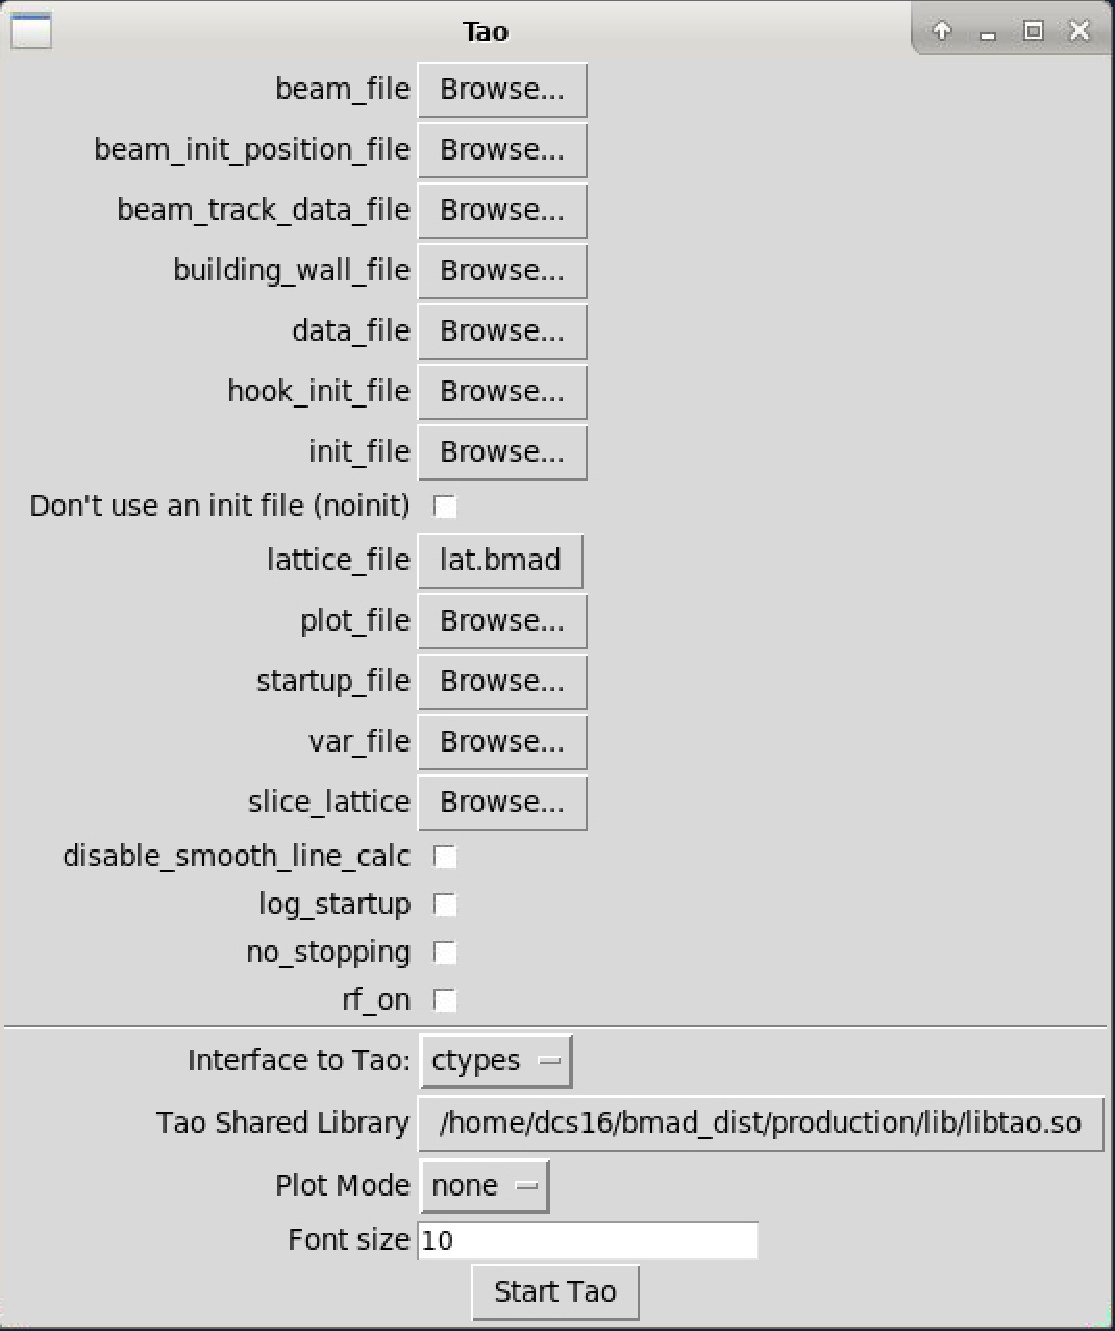
\includegraphics[width=8cm]{figures/startup.pdf}
\centering
\caption[The GUI startup window.]{The GUI startup window. In this example, the init file that tao should use has been specified.}
\label{fig:startup}
\end{figure}

%--------------------------------------------------------------
\section{GUI Initialization File}
\label{s:gui.init.file}

To speed up the initialization process, you can make an init file for the GUI.  This file should be called "gui.init", and it should be in the same directory from which you start the GUI.

gui.init should have each option on a separate line, and each option should be listed in the form "parameter:value".  For example, the text below would constitute a good gui.init file:
\begin{example}
  #MY GUI INIT FILE
  beam_file:/path/to/beam/file
  data_file:/path/to/data/file
  #THIS IS A COMMENT
  disable_smooth_line_calc:T
  rf_on:T
  tao_executable:/path/to/executable
\end{example}
For \tao specific parameters, The names in the \vn{gui.init} file correspond to the names in in the startup window
(\fig{fig:startup}). For GUI specific parameters (below the horizontal separator), replace blanks between words and
make all letters lower case. For example, ``\vn{Interface to Tao}'' in the startup window becomes \vn{interface_to_tao}
in the \vn{gui.init} file. Note: The startup window can be bypassed altogether by setting \vn{start_tao} in \vn{gui.init}
to \vn{True}.

The order in which you list options in gui.init is not important.

File paths should be specified in full to be safe, but you can specify paths relative to the directory from which you launch main.py.  For example, "/home/username/file", "subfolder/my_file", and "../../path/to/another/file" would all be acceptable file paths.  You can also use your environmental variables and "\textasciitilde{}", as in "\textasciitilde{}/Documents/my_file" and "\$DIST_BASE_DIR/tao/file".

For logical parameters, for example, "rf_on", Use T/F or True/False as the parameter's value.

You can also include comments with \#.  Anything after a \# character will be ignored.

To get a list of parameters that can be set in a \vn{gui.init} file, start Tao with the command
\begin{example}
  tao -help
\end{example}
The corresponding gui.init parameter is the Tao parameter with the leading dash "-" removed and a
colon ":" between the parameter and the parameter's value. 


\chapter{GUI Windows}

%-----------------------------------------------------------------
\section{Parameter Input}
\label{s:param.input}

In general, real parameter values can be set using expressions just like parameter values can be set
using expressions on the \tao command line.

%-----------------------------------------------------------------
\section{The Main GUI Window}
\label{s:gui.root.window}

\begin{figure}
\centering
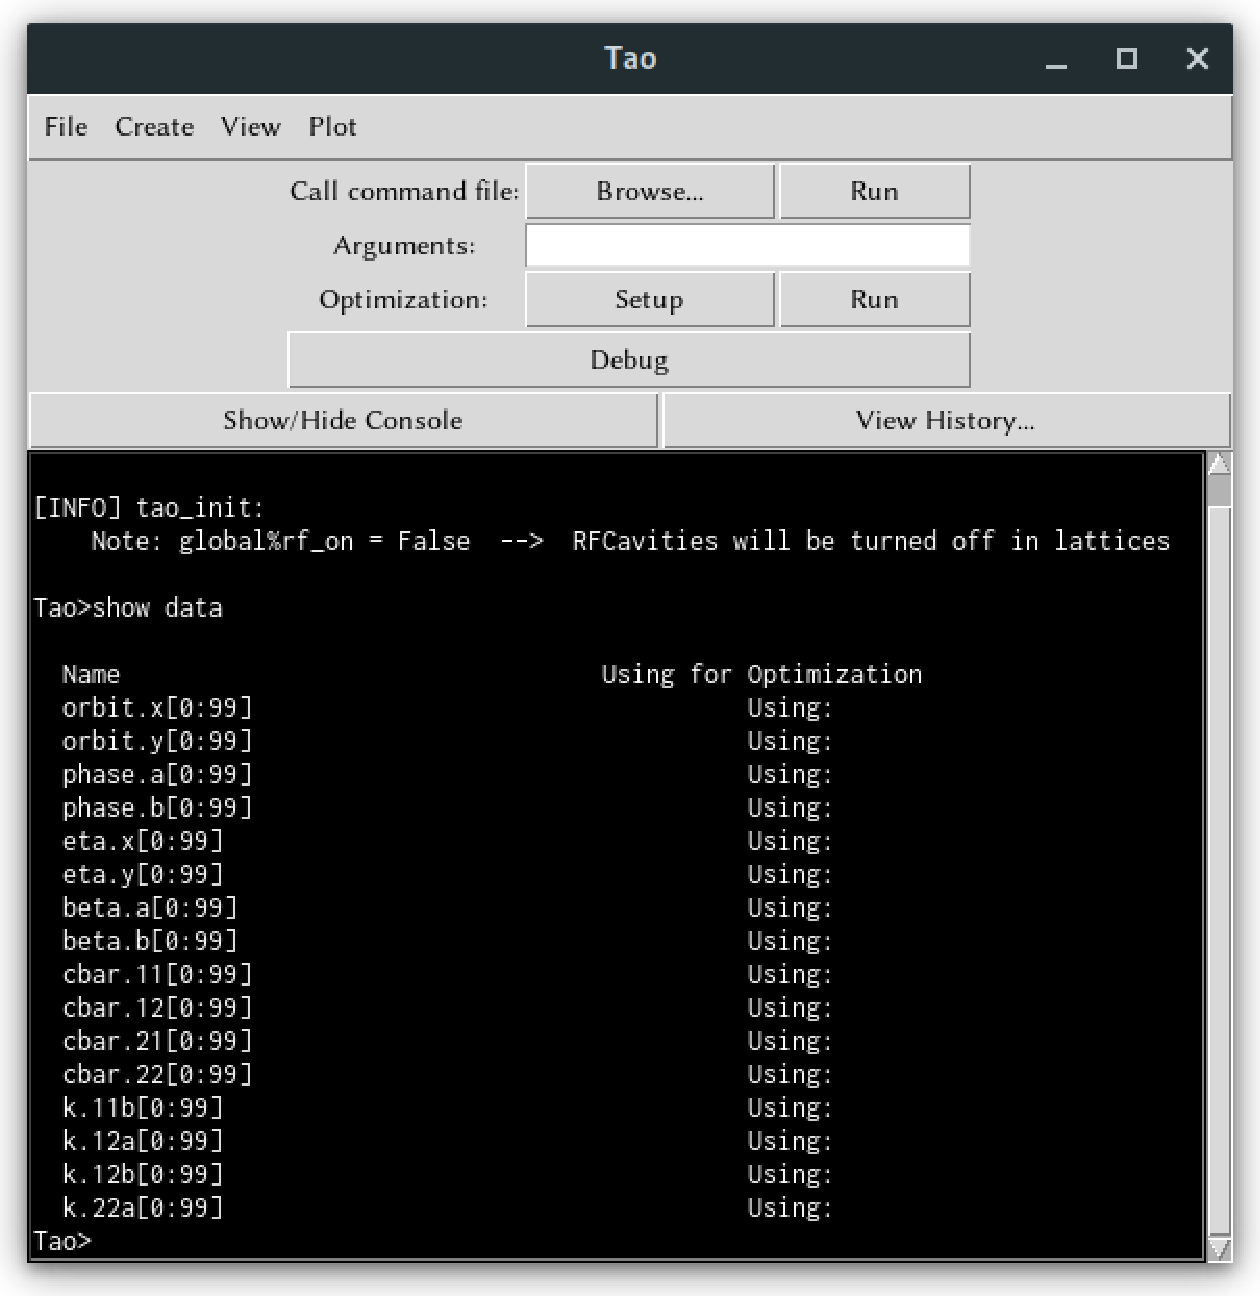
\includegraphics[width=8cm]{figures/root_window.pdf}
\caption[The main GUI window.]{The main GUI window, showing the results of \texttt{show data} on the console.}
\label{fig:root.window}
\end{figure}

The main window for the GUI is shown in Figure \ref{fig:root.window}.
From here, the user has access to all of the GUI's features.
Command files can be called by browsing for them and then clicking "Run", with arguments specified in the "Arguments" below.
In the future, the user will also be able to set up and run optimization routines from this window, although this feature is not currently available.

The main window also has a console, where commands can be run in Tao exactly like in regular Tao.
The console will also display warning messages if a command produces an error.

%-----------------------------------------------------------------
\section{Global Variables}
\label{s:gui.global.variables}

Global variables in Tao can be viewed and modified from the global variables window as shown in Figure \ref{fig:gui.global.variables}.
Once you have editted the global variables, clicking the "Set Global Variables" button will set the variables in Tao as appropriate.

\begin{figure}
\centering
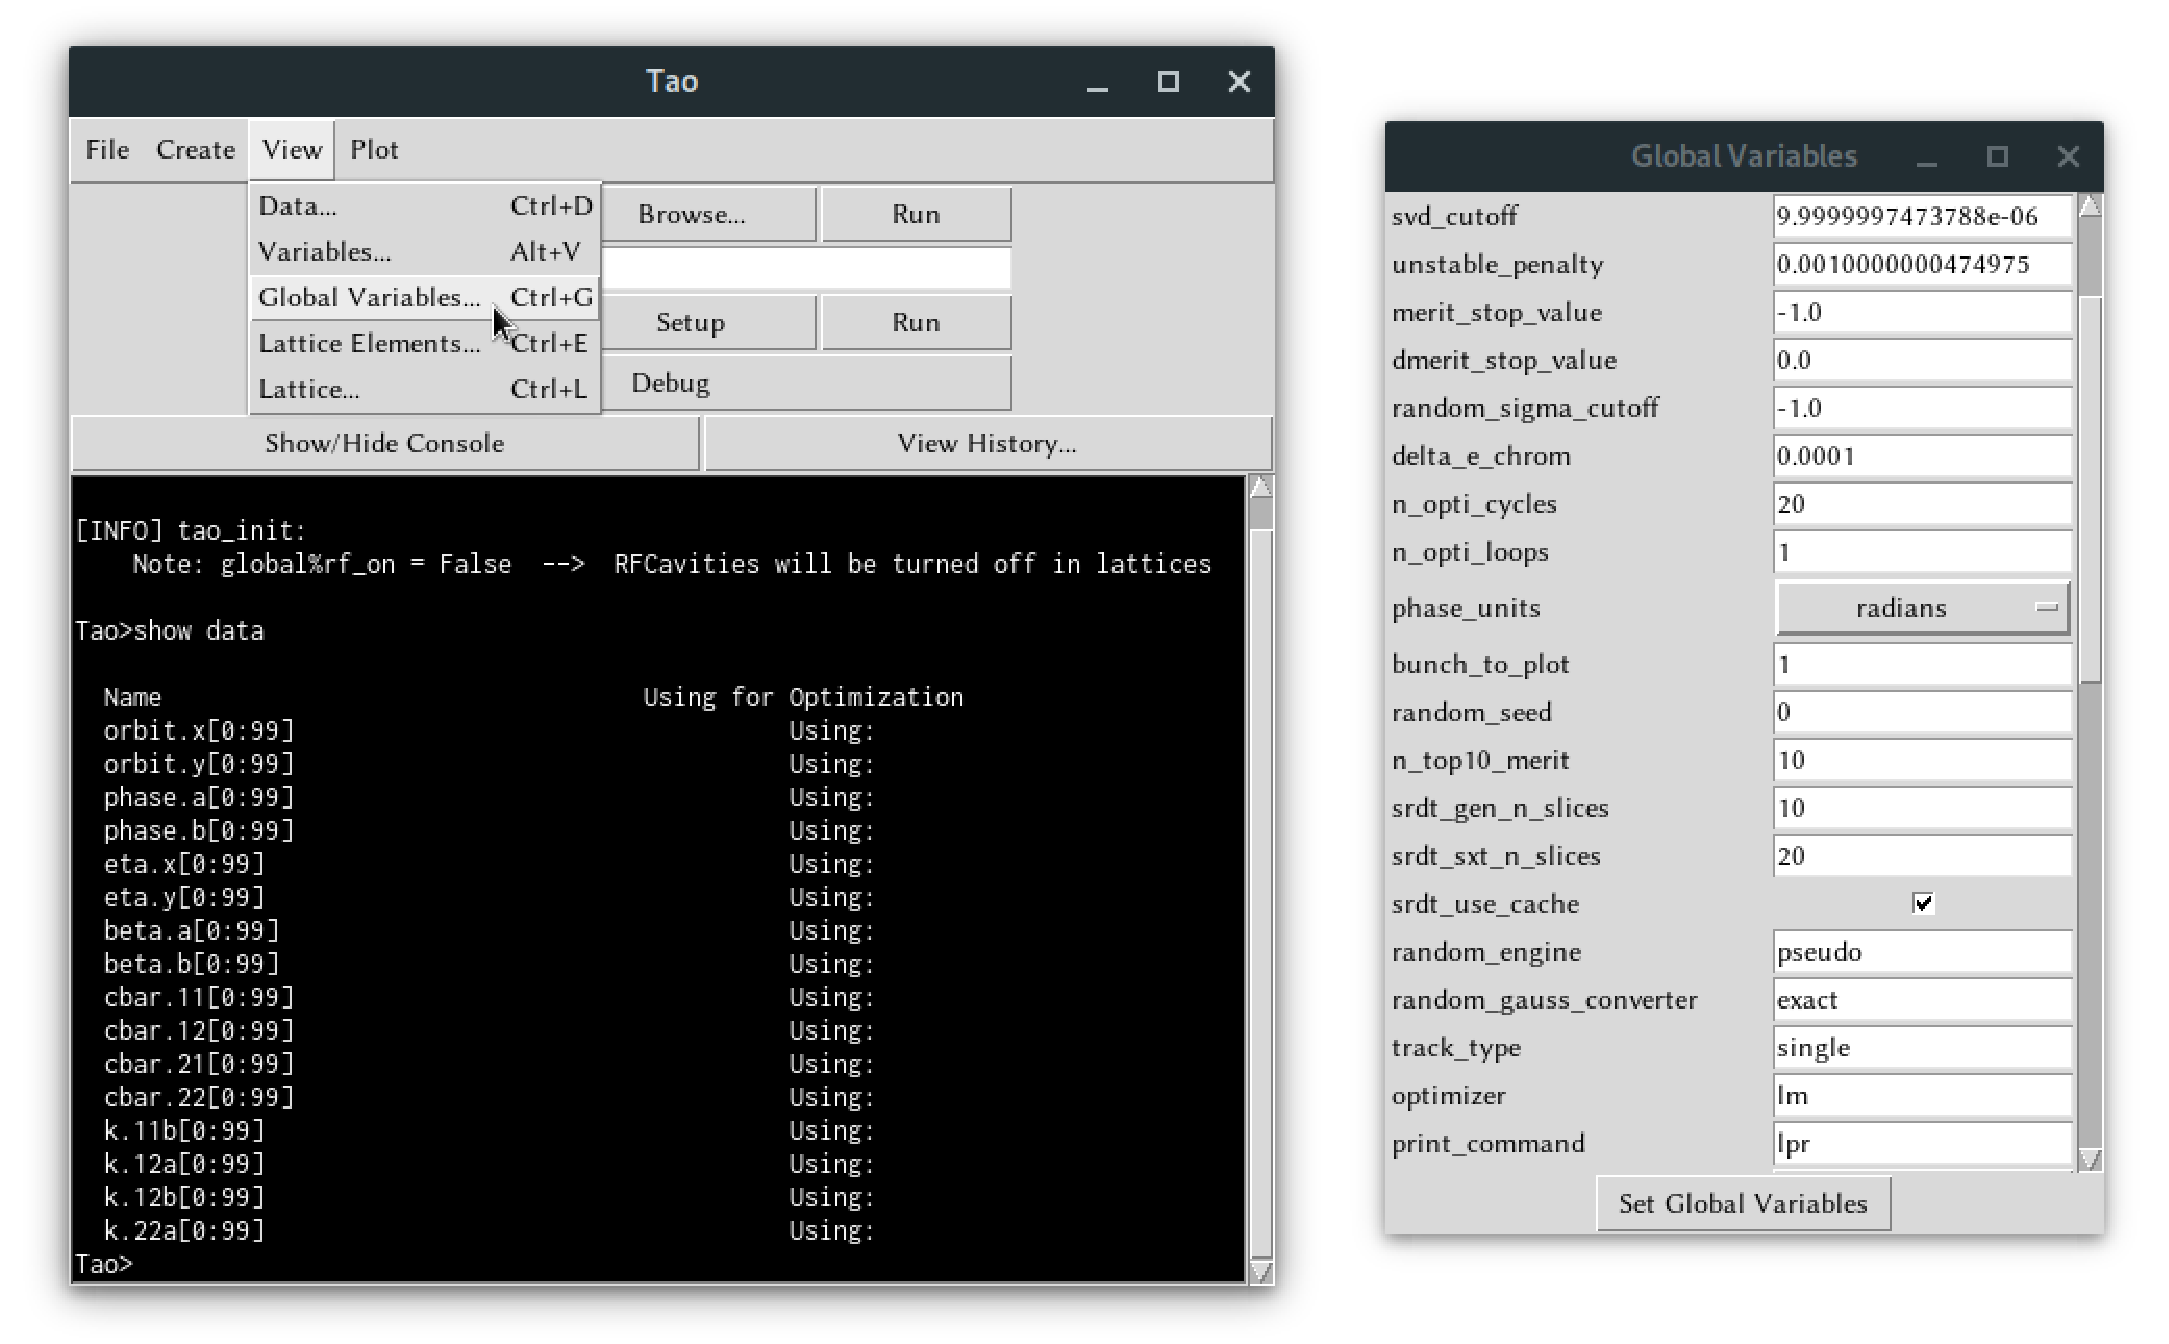
\includegraphics[width=10cm]{figures/globals.pdf}
\caption{View and edit global variables with the Global Parameters window.}
\label{fig:gui.global.variables}
\end{figure}


\chapter{Plotting}
\index{plotting}
\label{c:plotting}

\begin{figure}[b]
  \centering
  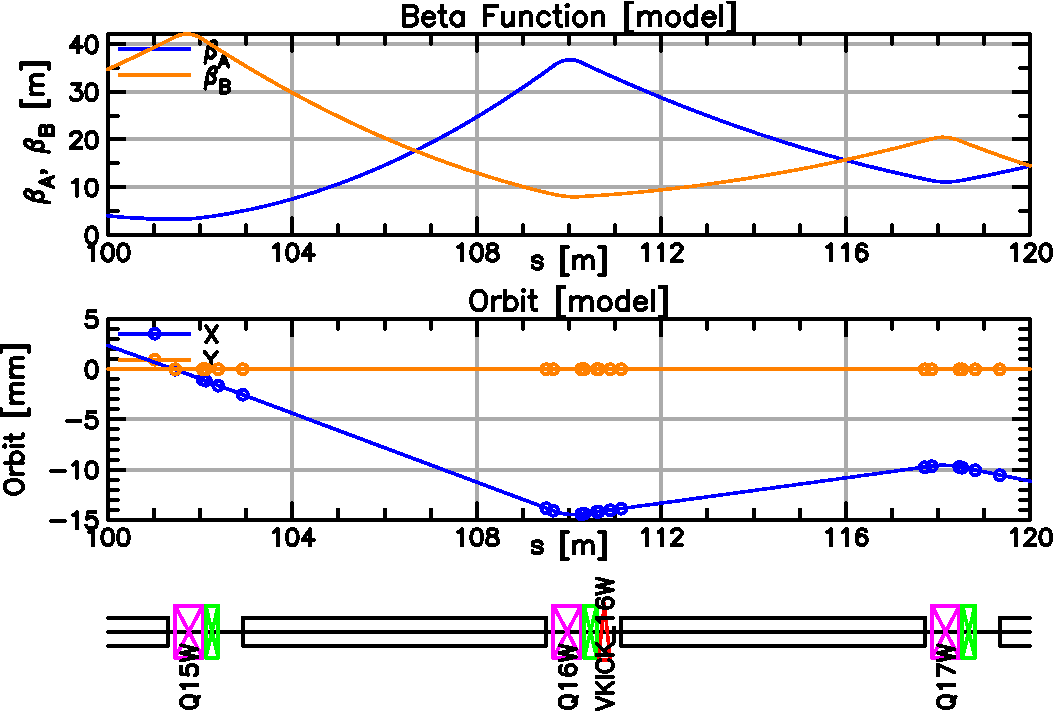
\includegraphics[width=4.5in]{plot-typical.pdf}
  \caption[An example of a plot display.]
{An example of a plot display. In this example there are three graphs: A graph displaying the beta
function, a graph displaying the orbit, and a graph displaying the ``lattice layout'' which shows
the longitudinal positions of lattice elements.}
  \label{f:plot.typ}
\end{figure}

\tao has a graphical display window within which such things as lattice functions, machine layout,
beam positions, etc., can be plotted. An example is shown in \fig{f:plot.typ} where there are plots
of the beta function and orbit along with a ``lattice layout which shows the longitudinal positions
of lattice elements. 

\tao organizes the display window using a number of concepts which are explained in the 
sections below
\begin{example}
  plot_page     ! The display window containing the graphics (\sref{s:plot.page.def}).
  regions       ! A set of rectangles on the plot_page that plots can be put in (\sref{s:region.def}).
  plot          ! A collection of graphs (\sref{s:plot.def}).
  box           ! Rectangular area within a plot that a graph is placed in (\sref{s:box.def}).
  graph         ! A diagram of some sort (\sref{s:graph.def}).
  curve         ! Data displayed within a \vn{graph} (\sref{s:curve.def}).
\end{example}

Underlying all this is the \vn{quick_plot} software toolkit (\sref{s:quick.plot}) which was developed
for \bmad and \tao for graphics plotting.

%-----------------------

\begin{figure}[bt]
  \centering
  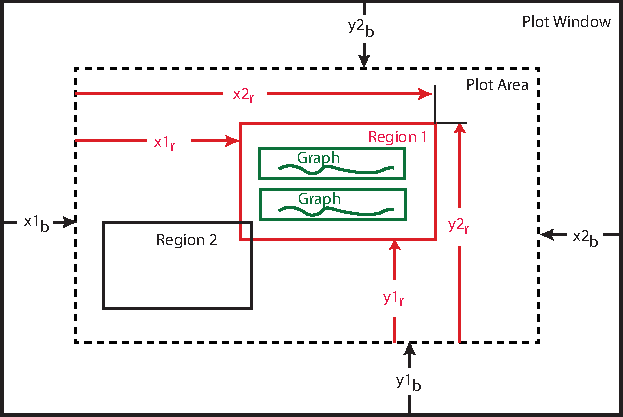
\includegraphics{plot-page.pdf}
  \caption[The plot window.]{The \vn{plot page} is the entire display window area. The \vn{plot area} 
is the region within the boarders of the \vn{plot page} within which ``\vn{regions}'' are
placed. The location of a \vn{region} is defined by four offsets with respect to the \vn{plot
area}. Regions may overlap.}
  \label{f:plot.page}
\end{figure}

%-----------------------------------------------------------------
\section{Plot Page}
\label{s:plot.page.def}

The \vn{plot page}, sometimes called the \vn{plot window}, refers to the window or the corresponding
printed graphics page where graphics are displayed. A \vn{plot page} is shown schematically in
\fig{f:plot.page}. Parameters associated with the \vn{plot page} are discussed in
\sref{s:plot.page}.  These parameters may be set in an initialization file or may be set on the \tao
command line using the \vn{set plot_page} (\sref{s:set.plot.page}) command. Examples:
\begin{example}
  set plot_page text_height = 11  ! 11 point font size
  set plot_page border%x1 = 0.2   ! Set left page border to 20% of width.
\end{example}

The size of the \vn{plot page} is set by the \vn{plot_page%size} parameter which is an array of two
numbers which set the width and height. The \vn{plot page} size can also be set when invoking \tao
using the \vn{-geometry} option (\sref{s:command.line})
\begin{example}
  > tao -lattice lat.bmad -geometry 300x500
\end{example}
This starts \tao with the \vn{plot page} size set to 300 points wide by 500 points high. It is also
sometimes convenient to start \tao without the plotting window. In this case, the \vn{-noplot} option
can be used on the startup command line. In a \tao initialization file, display of the plot window can be set
using the \vn{global%plot_on} parameter set in the \vn{tao_params} namelist (\sref{s:globals}).

The \vn{plot page} has a border within which \vn{regions} (\sref{s:region.def}) are defined. The area withing
the plot page border is called the \vn{plot area}

The \vn{show plot -page} (\sref{s:show.plot}) command may be used to view the page parameters.

%-----------------------------------------------------------------
\section{Region}
\label{s:region.def}

The \vn{plot area} is the area within the border of the \vn{plot page} as shown in
\fig{f:plot.page}.  In this \vn{plot area}, ``\vn{regions}'' can be defined which are invisible
rectangles where a \vn{plot} (\sref{s:plot.def}) can be placed. This is shown schematically in
\fig{f:plot.page}. Each region has a name and four numbers which specifies the location of the
region within the plot area. Regions may be defined by the user. In addition, for convenience, \tao
will define a number of regions. \tao defined regions will either begin with the letter ``\vn{r}''
or begin with the string ``\vn{layout}'' or the string ``\vn{scratch}''. Regions may overlap. How to
define regions is explained in \sref{s:plot.page}. The \vn{show plot} command will show the region
list. Example:
\begin{example}
  Tao> show plot

Plot Region         <-->  Plot                 x1    x2    y1    y2     Visible
-----------               -----------------------------------------------------
layout              <-->  lat_layout          0.00  1.00  0.00  0.15         T
r11                 <-->                      0.00  1.00  0.15  1.00
r12                 <-->                      0.00  1.00  0.58  1.00
r22                 <-->                      0.00  1.00  0.15  0.58
r13                 <-->  beta                0.00  1.00  0.72  1.00         T
r23                 <-->  dispersion          0.00  1.00  0.43  0.72         T
r33                 <-->  orbit               0.00  1.00  0.15  0.43         T
r14                 <-->                      0.00  1.00  0.79  1.00
\end{example}
The \vn{Plot} column shows what \vn{plot} (if any) is associated with the region
(\sref{s:plot.def}). The next four columns show the values of \vn{x1}, \vn{x2}, \vn{y1}, and \vn{y2}
set for the region. As shown in \Sref{s:plot.page}, \vn{x1} and \vn{x2} are the offsets from the
left \vn{plot area} edge to the left and right edges of the region. Similarly, \vn{y1} and \vn{y2}
are the offsets from the bottom edge of the \vn{plot area} to the bottom and top edges of the
region. \vn{x1} and \vn{x2} are normalized by the \vn{plot area} width and \vn{y1} and \vn{y2} are
normalized by the \vn{plot area} height so all four numbers should be in the range $[0, 1]$.  Using
the above example, the \vn{r23} region spans the full width of the \vn{plot area} (since \vn{x1} = 0
and \vn{x2} = 1), and occupies approximately the middle third vertically of the \vn{plot area}
(since \vn{y1} = 0.43 and \vn{y2} = 0.72).

The last column in the above shows if the \vn{plot} associated with the \vn{region} is
visible. Normally everything is visible. Invisibility is used in some special cases. For example,
when using a Graphical User Interface (GUI).

The \vn{set region} command can be used to set region parameters. Example:
\begin{example}
  set region r13 y1 = 0.8  ! Sets lower edge vertical position
\end{example}

%-----------------------------------------------------------------
\section{Plot}
\label{s:plot.def}

A \vn{plot} is essentially a collection of \vn{graphs}. This is shown schematically in
\fig{f:plot.plot} which shows a plot with two graph side by side.

Plots are divided into two groups. A \vn{template} plot defines how a \vn{displayed} plot is to be
constructed. That is, a \vn{template} plot defines what the associated \vn{graphs} are, defines
graph placement within the plot, etc. When a \vn{template} plot is \vn{placed} in a \vn{region},
either by using the \vn{place} command (\sref{s:place}) or by placement defined in an initialization
file (\sref{s:plot.page}), the information of the \vn{template} is copied in order to construct a
\vn{displayed} plot. A given \vn{template} plot may be placed in multiple \vn{regions} to give
multiple \vn{displayed} plots and then, using \vn{set} commands, the data displayed in each of these
plots may be manipulated separately. For example, one displayed orbit plot could show the orbit of
the \vn{model} lattice while another orbit plot could show the orbit difference between the
\vn{model} and \vn{design} lattices. When a \vn{plot} is displayed in a given \vn{region},
everything drawn is scaled to the region size.

Use the \vn{show plot} to see what displayed plots are associated with what regions. Use the
\vn{show plot -templates} command to see a list of \vn{template} plots. \tao defines a number of
default \vn{template} plots. Section~\sref{s:template} discusses how to define custom template
plots in an initialization file. Use the \vn{set plot} command (\sref{s:set.plot}) to modify either
\vn{template} or \vn{displayed} plots.

All plots have a name. A \vn{displayed} plot will inherit the same name of the \vn{template} plot it
came from. If a given \vn{template} plot is used to create multiple \vn{displayed} plots. All of
these plots will have the same name. A \vn{displayed} plot can also be referred to by using the
associated \vn{region} name. This can be used to remove ambiguity if there are multiple
\vn{displayed} plots of the same name. Additionally, a \vn{template} plot can unambiguously be
referred to by adding the prefix ``\vn{T::}'' to the plot name. Examples:
\begin{example}
  show plot           ! Show plots associated with regions
  show plot -template ! Show template plots
  place r13 orbit     ! Put orbit template into r13 region
\end{example}

Some commands, for example, the \vn{scale} command by default will ignore \vn{template} plots unless
the plot name has the \vn{T::} prefix. Other commands, for example the \vn{show plot} command, will
preferentially show displayed plot info but will show template plot info if there are no matching
displayed plots. Examples:
\begin{example}
  scale orbit -10 10    ! Scale all displayed orbit plots. Ignore template.
  scale r33 -10 10      ! Scale only plot in r33 region.
  scale T::orbit -10 10 ! Scale template orbit plot.
  show plot e_field     ! Will show displayed e_field plot info. If no
                        ! displayed plot exists, will show template info.
\end{example}

%-----------------------

\begin{figure}[bt]
  \centering
  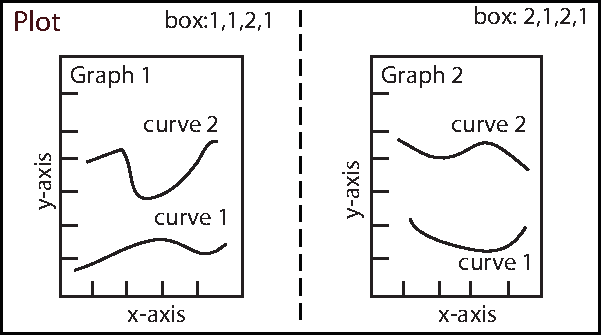
\includegraphics[width=5.0in]{plot-plot.pdf}
  \caption[Plotting nomenclature.]
  {
A plot has a collection of graphs and a graph has a collection of curves. A graph is located within
a plot by defining the ``\vn{box}'' associated with the \vn{graph}. Illustrated here is a plot with
two graphs placed side by side.
  }
  \label{f:plot.plot}
\end{figure}

%-----------------------------------------------------------------
\section{Box}
\label{s:box.def}

To determine where a \vn{graph} is drawn with respect to the boundaries of its associated \vn{plot},
each \vn{graph} is associated with a given ``\vn{box}''. A \vn{box} is a rectangular sub-region of
the \vn{plot}. Boxes are defined by dividing the \vn{plot} into a rectangular grid and then choosing
one of the grid rectangles to be the \vn{box} associated with the \vn{graph}. The is illustrated in
\fig{f:plot.plot} where \vn{Graph 1} is associated with the \vn{box} labeled ``\vn{1,1,2,1}'' and
\vn{Graph 2} is associated with the \vn{box} labeled \vn{2,1,2,1}.  The last two digits of a
\vn{box} label (\vn{2,1} for both graphs) specify the number of rectangles the grid has horizontally
and vertically (2 horizontally, 1 vertically here). The first two digits (\vn{1,1} for \vn{graph 1}
and \vn{2,1} for \vn{graph 2}) specify the particular rectangle associated with the \vn{box} with
\vn{1,1} designating the lower left rectangle. Different \vn{graphs} do not have to use the same
grid division to select a box from.

Setting the \vn{box} for a given \vn{graph} in a \tao initialization file is covered in \sref{s:template}.
The \vn{set graph} and \vn{show graph} commands can be used to set and show the box parameters. 
Examples:
\begin{example}
  set graph myplot.g1 box = 2 1 2 2  ! Set box of graph myplot.g1
  set graph myplot.g2 box = 1 1 1 2  ! Different graphs can use different grids
                                     !  for box selection
\end{example}

%-----------------------------------------------------------------
\section{Graph}
\label{s:graph.def}

%-----------------------------------------------------------------
\subsection{Overview}
\label{s:graph.overview}

A \vn{graph} is a diagram of some sort. Most \vn{graph}s consists of horizontal and vertical axes
along with one or more \vn{curve}s. \vn{Floor_plan} (\sref{s:floor.plan}) and \vn{lat_layout}
(\sref{s:lat.layout}) \vn{graphs}, on the other hand, shows the placement in space of the lattice
elements and do not have any associated \vn{curves}.

Every \vn{plot} has at least one \vn{graph}. How many \vn{graphs} are associated with a \vn{plot}
is a matter of convenience and different \vn{graphs} of a \vn{plot} may display different types of
information. For example, it would be possible to have a single \vn{plot} contain three \vn{graphs}
and look like what is shown in \fig{f:plot.typ}. In actuality, the figure was constructed using
three \vn{plots} each one containing one \vn{graph}.

How to define \vn{graphs} when defining \vn{template} plots is given in \sref{s:template}. The
\vn{show graph} command can be used to show graph parameters. The \vn{set graph} command can
be used to modify \vn{graph} parameters.

%-----------------------------------------------------------------
\subsection{Graph Name}
\label{s:graph.name}

All graphs have a name. For example, the graph of the standard \vn{orbit} plot is simply ``\vn{g}''.
\vn{Graphs} may be referred to using the syntax:
\begin{example}
  <plot>.<graph>
\end{example}
where \vn{<plot>} is the plot name (or the \vn{region} name associated with the \vn{plot}) and
\vn{<graph>} is the graph name. If the \vn{.<graph>} ending is omitted, all graphs of the named
\vn{plot}(s) are selected. Examples:
\begin{example}
  show graph beta   ! Show info of all graphs in all the displayed beta plots.
  show graph r13.g1 ! Show info on ``g1'' graph of region r13.
\end{example}

%-----------------------------------------------------------------
\subsection{Curve Legend of a Graph}
\label{s:curve.legend}

The \vn{curve legend} is the legend identifying what curves are associated with what perimeters. In
\fig{f:plot.typ} the top two graphs have a curve legend in the upper left hand corner of the graph.
By default, the \vn{data_type} of each curve will be used as the text for that
curve's line in the legend.  This default can be changed by setting a curve's \vn{curve%legend_tex}.
Parameters that affect the curve legend are:
\begin{example}
  plot_page%legend_text_scale        
  plot_page%curve_legend_line_len    ! tao_plot_page namelist (\sref{s:plot.page})
  plot_page%curve_legend_text_offset ! tao_plot_page namelist (\sref{s:plot.page})
  curve(N)%legend_text               ! 
  graph%curve_legend_origin          
  graph%draw_curve_legend            
\end{example}
The curve legend is distinct from the \vn{text legend} (\sref{s:text.legend}).

%-----------------------------------------------------------------
\subsection{Text Legend}
\label{s:text.legend}

The \vn{text legend} is a legend that can be setup by either the user or by \tao itself.
\tao uses the text legend in conjunction with phase space plotting or histogram displays.
The \vn{text legend} is distinct from the \vn{curve legend}. Parameters that affect the text
legend are:
\begin{example}
  graph%text_legend(N)
  graph%text_legend_origin
\end{example}

%-----------------------------------------------------------------
\subsection{Graph Types}
\label{s:graph.types}

\tao defines several kinds of graphs. The \vn{graph%type} in the \vn{tao_template_graph}
(\sref{s:template}) sets the type.
\begin{description}
%
\item["data"] \Newline
``Data'' plotting is the plotting of a dependent variable on the $y$-axis vs an independent variable
on the $x$-axis. Typically the independent variable will be the longitudinal position $s$-position
as in the upper two graphs in \fig{f:plot.typ}. Also see \Sref{s:draw.ap} for an example where beam
apertures are added to the graph.

A ``\vn{data slice}'' graph is plotting one data array on the $y$-axis versus another data array on
the $x$-axis (\sref{s:graph.data.slice}). Also see \vn{parametric plotting} (\sref{s:param.plot}).

With a \vn{parametric} plot both the $x$ and $y$ values of the points on a curve are dependent
upon an independent parameter (\sref{s:param.plot}). This is similar to a \vn{data slice} plot
(\sref{s:graph.data.slice}).
%
\item["dynamic_aperture"] \Newline
A \vn{dynamic aperture} graph (\sref{s:da.plot}) draws the results from a dynamic aperture
calculation (\sref{s:da.calc}).
%
\item["floor_plan"] \Newline
A \vn{floor plan} graph shows the physical layout of the machine (\sref{s:floor.plan}). A table maps
lattice elements to a shape that is drawn (\sref{s:shapes}). The user may override the default
mapping. Besides the lattice elements. the outline of the building or tunnel that the machine is in
can be drawn (\sref{s:building.wall}).
%
\item["histogram"] \Newline
Currently \vn{histograms} (\sref{s:histogram}) are limited to displaying phase space data.
%
\item["key_table"] \Newline
The \vn{key table} displays information about variables bound to keyboard keys \sref{s:key.bind}.
Key bindings are used in \vn{single mode}.
%
\item["lat_layout"] \Newline
A \vn{lattice layout} graph displays the lattice elements as a series of shapes as a function of the
longitudinal position $s$ (\sref{s:lat.layout}). The lowest graph in \fig{f:plot.typ} is an example
of a \vn{lattice layout}.  A table maps lattice elements to a shape that is drawn (\sref{s:shapes}).
The user may override the default mapping.
%
\item["phase_space"] \Newline
A \vn{phase space graph} (\sref{s:phase.space}) displays particle positions in phase space after
a beam of particles has been tracked (\sref{s:beam.init}).
%
\item["wave.0", "wave.a", "wave.b"] \Newline
Wave analysis plotting (\sref{c:wave}).
%
\end{description}

\begin{figure}[b]
  \centering
  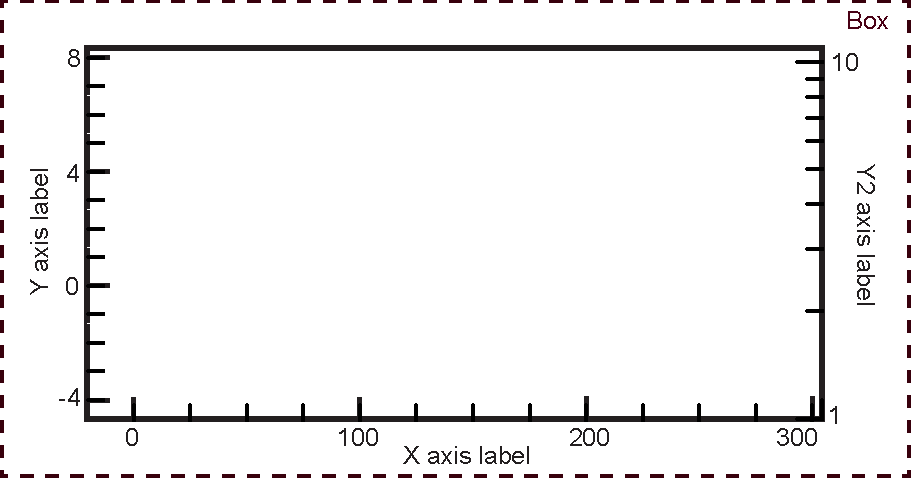
\includegraphics[width=5.0in]{plot-axes.pdf}
  \caption[Plot axes.]
{A data graph has three axes called \vn{x} (bottom edge), \vn{y} (left edge), and \vn{y2} (right edge).}
  \label{f:plot.axes}
\end{figure}

%-----------------------------------------------------------------
\subsection{Graph Axes}
\label{s:axes}

Data graphs (\sref{s:graph.types}) have three axes as shown in \fig{f:plot.axes}. The bottom axis is
called \vn{x}, and the left and right axes are called \vn{y} and \vn{y2} respectively. The \vn{qp_axis_struct}
structure (\sref{s:qp.axis}) is used to store axis parameters.

The \vn{scale} command (\sref{s:scale}) can be used to set the vertical axes. The \vn{x_scale}
(\sref{s:x.scale}) command can be used to set the horizontal axis.

Normally there is only one vertical scale for a graph and this is associated with the \vn{y}
axis. However, if any curve of a given graph has \vn{curve%use_y2} set to \vn{True} then the \vn{y2}
axis will have an independent second scale. In this case, the \vn{y2} axis numbers will be
drawn. Notice that simply giving the \vn{y2} axis a label does {\em not} make the \vn{y2} axis scale
independent of the \vn{y} axis scale.

%-----------------------------------------------------------------
\section{Curve}
\label{s:curve.def}

%-----------------------------------------------------------------
\subsection{Overview}
\label{s:curve.overview}

A \vn{curve} is a data set to be displayed within a \vn{graph}. For example, a \vn{curve} may be the
beta function of the \vn{model} lattice. \vn{Curves} have an associated set of points at which a
symbol can be drawn. A curve also can have an associated curved line that can be drawn. For example,
in \fig{f:plot.typ} only the line is drawn with the two curves of the beta plot while both symbols
and line are drawn for the two curves of the orbit plot (here the data points where symbols are
drawn are the orbit at the edges of the lattice elements).

Some \vn{graphs} do not have any associated curves. For example, a \vn{lat_layout} graph does not
have associated curves.

How to define \vn{curves} when defining \vn{template} plots is given in \sref{s:template}. The
\vn{show curve} command can be used to show curve parameters. The \vn{set curve} command can
be used to modify \vn{curve} parameters.

%-----------------------------------------------------------------
\subsection{Curve Name}
\label{s:curve.name}

All curves have a name. \vn{Curves} may be referred to using the syntax:
\begin{example}
  <plot>.<graph>.<curve>
\end{example}
where \vn{<plot>} is the plot (or \vn{region}) name, \vn{<graph>} is the graph name and \vn{<curve>}
is the curve name. If the \vn{.<curve>} ending is omitted, all curves of the named \vn{graph}(s) are
selected. If the \vn{.<graph>.<curve>} ending is omitted, all curves of the named \vn{plot}(s) are
selected. Examples:
\begin{example}
  show curve beta   ! Show info of all curves in all the displayed beta plots.
  show curve r13.g1 ! Show info on curves in ``g1'' graph of region r13.
  set graph orbit.g curve_legend_origin = 0.1 -0.2 "%BOX/LT"  ! Set curve legend origin
\end{example}
The last example sets the \vn{curve legend} (\sref{s:template}) of the graph so that the curve
legend of the graph is drawn with respect to the left top corner of the box.

%-----------------------------------------------------------------
\subsection{Curve Line}
\label{s:curve.line}

Each curve may have an associated line that is drawn. The line may be a set of line segments
connecting curve symbol points (\sref{s:curve.sym}) or may be a ``smooth'' curve calculated by
evaluating the curve at a number of points. 

\vn{curve%draw_line} determines whether a curve is drawn through the data point symbols. The
thickness, style (solid, dashed, etc.), and color of the line can be controlled by setting
\vn{curve%line}. If \vn{plot%x_axis_type} is \vn{"s"}, and \vn{curve%component} does not contain
\vn{"meas"} or \vn{"ref"}, \tao will attempt to calculate intermediate values in order to draw a
smooth, accurate curve is drawn. Occasionally, this process is too slow or not desired for other
reasons so setting \vn{curve%smooth_line_calc} to False will prevent this calculation and the curve
will be drawn as a series of lines connecting the symbol points. The default of
\vn{curve%smooth_line_calc} is True. Use the \vn{set curve} command (\sref{s:set}) to toggle the
drawing of lines. Alternatively, the \vn{-disable_smooth_line_calc} switch can be used on the
command line (\sref{s:command.line}) or the global variable \vn{global%disable_smooth_line_calc} can
be set in the \tao initialization file (\sref{s:globals}).

The number of points to evaluate at when constructing a smoothed line is set by
\vn{plot_page%n_curve_pts} in the \vn{tao_plot_page} namelist (\sref{s:plot.page}) or by using the
\vn{set plot_page} command (\sref{s:set.plot.page}). To override this value for a particular plot
the \vn{plot%n_curve_pts} parameter can be set in the \vn{tao_template_plot} namelist or using the
\vn{set plot} command (\sref{s:set.plot}). More evaluation points may give a more accurate curve at
the expense of computation time.

%-----------------------------------------------------------------
\subsection{Curve Symbol}
\label{s:curve.sym}

\vn{curve%draw_symbols} determines whether a symbol is drawn at the data points. The size, shape and
color of the symbols is determined by \vn{curve%symbol}. A given symbol point that is drawn has
three numbers attached to it: The $(x, y)$ position on the graph and an index number to help
identify it. The index number of a particular symbol is the index of the datum or variable
corresponding the symbol in the \vn{d1_data} or \vn{v1_var} array. These three numbers can be
printed using the \vn{show curve -symbol} command (\sref{s:show}).  \vn{curve%draw_symbol_index}
determines whether the index number is printed besides the symbol. Use the \vn{set curve} command
(\sref{s:set}) to toggle the drawing of symbols. The default value for \vn{curve%draw_symbol} is
False if \vn{plot%x_axis_type} is \vn{"s"}, \vn{"curve"}, \vn{"lat"}, or \vn{"var"} and True
otherwise. The default \vn{curve%draw_symbol_index} is always False.

The \vn{graph%draw_only_good_user_data_or_vars} logical determines whether datums
(\sref{s:init.data}) or variables (\sref{s:init.var}) with a \vn{good_user} component set to
\vn{False} are drawn. The default is to not draw them which means that data or variables not used in
an optimization are not drawn.

%-----------------------------------------------------------------
\subsection{Curve Component}
\label{s:curve.comp}

A ``\vn{data}'' graph (\sref{s:graph.types}) is used to draw lattice parameters such as orbits, or
\tao data (\sref{c:data}), or variable values such as quadrupole strengths. The data values will
depend upon where the data comes from. This is determined, in part, by the setting of the
\vn{component} parameter in the \vn{tao_template_graph} namelist (\sref{s:template}).  The
\vn{component} may be one of:
\index{model}\index{design}\index{base}\index{meas}\index{ref}
\begin{example}
  "model"             ! model values. Default.
  "design"            ! design values.
  "base"              ! Base values
  "meas"              ! data values.
  "ref"               ! reference data values.
  "beam_chamber_wall" ! Beam chamber wall
\end{example}
Additionally, \vn{component} may be set to plot a linear combination of the above. For
example:
\begin{example}
  &tao_template_graph
    curve(2)%component = "model - design"
    ...
\end{example}
This will plot the difference between the \vn{model} and \vn{design} values. 
The default value of \vn{%component} is \vn{"model"}.

%-----------------------------------------------------------------
\subsection{Curve Data Source}
\label{s:curve.source}

\index{data}\index{var}\index{calculation}
\index{curve!data_source}
The \vn{data_source} parameter of a curve is the type of information for the source of the data points.
\vn{data_source} must be one of:
\begin{example}
  "data"              ! A d1_data array is the source of the curve points.
  "var"               ! A v1_var array is the source of the curve points.
  "lat" (Default)     ! The curve points are computed directly from the lattice.
  "beam"              ! The curve points are computed from tracking a beam of particles.
  "multi_turn_orbit"  ! Computation is from multi-turn tracking. 
\end{example}
The default for \vn{data_source} is \vn{"lat"}. With \vn{data_source} set to "\vn{data}",
the values of the curve points come from the \vn{d1_data} array structure named by
the curve's \vn{data_type} parameter (\sref{s:curve.type}).

If \vn{data_source} is set to \vn{var}, the values of the curve points come from a \vn{v1_var}
array structure. If it is set to \vn{lat} the curve data points are calculated from the lattice
without regard to any data structures. \vn{data_source} can be set to \vn{beam} when tracking
beams of particles. In this case, the curve points are calculated from the tracking. With \vn{beam},
the particular bunch that the data is extracted from can be specified via \vn{ix_bunch}. The
default is \vn{0} which combines all the bunches of the beam for the calculation.

Used in conjunction with \vn{data_type} and \vn{component} (\sref{s:curve.comp}). For
example (\sref{s:curve.source}), a curve of the orbit with \vn{data_source} set to \vn{"beam"}
would use the beam centroid computations. If the \vn{data_source} was set to \vn{"lat"} the
computed orbit using single particle tracking is used.

Example: With \vn{data_type} set to \vn{beta.x}, the setting of \vn{data_source} to
\vn{lat} gives the beta as calculated from the lattice and \vn{beam} gives the beta as calculated
from the shape of the beam.

%-----------------------------------------------------------------
\subsection{Curve Data Type}
\label{s:curve.type}

The \vn{data_type} of a curve specifies what is being plotted. What the valid settings for \vn{data_type}
are depends upon the type of graph (\sref{s:graph.types}). 
\begin{description}
%
\item[graph\%type = "data", or "histogram"] \Newline
Valid settings for \vn{data_type} are any \tao datum type (\sref{s:data.table}), \tao variable
(\sref{c:var}), and the following electric and magnetic field components:
\begin{example}
  b0_field.x,  b0_field.y,  b0_field.z,  b0_curl.x,  b0_curl.y,  b0_curl.z,  b0_div
  e0_field.x,  e0_field.y,  e0_field.z,  e0_curl.x,  e0_curl.y,  e0_curl.z,  e0_div
\end{example}
The field data types with names starting with ``b_'' and ``e_'' evaluate the field along the single
particle trajectory while the field data types with names starting with ``b0_'' and ``e0_'' are evaluated
along a constant transverse position specified by the curve's \vn{orbit} parameter.
%
\item[graph\%type = "dynamic_aperture"] \Newline
Valid settings for \vn{data_type} are:
\begin{example}
  "beam_ellipse"
  "dynamic_aperture"
\end{example}
%
\item[graph\%type = floor_plan", "lat_layout", or "key_table"] \Newline
There are not curves associated with these graph types.
%
\item[graph\%type = "phase_space"] \Newline
Valid settings for \vn{data_type} are:
\begin{example}
  "x",  "px",  "y",  "py",  "z",  "pz",
  "intensity",  "intensity_x",  "intensity_y"     ! Photon intensity
  "phase_x", "phase_y"                            ! Photon coherent phase
\end{example}
%
\end{description}

 For example, with \vn{graph%type} set to
\vn{dynamic_aperture} the 




Thus in the above example the curve point values are obtained from
\vn{orbit.x} data. To be valid the data structure named by \vn{data_type} must be set up in an
initialization file. If not given, the default \vn{data_type} is
\begin{example}
  <plot%name>.<graph%name>
\end{example}

%-----------------------------------------------------------------
\section{Quick_Plot Plotting}
\label{s:quick.plot}

\vn{Quick_plot} is a software library developed for \bmad and \tao for graphics plotting.

%-----------------------------------------------------------------
\subsection{Length and Position Units}
\label{s:qp.units}

Positions and lengths with \vn{quick_plot} generally have an associated ``\vn{units}'' string which determines how
$(x, y)$ positions or $(dx, dy)$ lengths are to be interpreted. 
The syntax of the \vn{units} parameter is:
\begin{example}
  "unit_type/ref_object/corner"
\end{example}
A \vn{units} string has a \vn{unit_type}, \vn{ref_object} and \vn{corner} components separated by slashes ``/''.

The \vn{unit_type} component is the type of units which can be one of:
\begin{example}
   "%"       - Percent.
   "DATA"    - Data units associated with a graph.
   "MM"      - millimeters.
   "INCH"    - Inches.
   "POINTS"  - Printers points (72 points = 1 inch, 1 pt ~ 1 pixel).
\end{example}
Note: If \vn{unit_type} is set to \vn{"DATA"}, \vn{ref_object}, if present, must be \vn{"GRAPH"} and
\vn{corner}, if present, must be \vn{"LB"}.

The \vn{ref_object} component is a reference object which can be one of:
\begin{example}
   "PAGE"  -- Relative to the plot display window.
   "BOX"   -- Relative to the box the graph is associated with.
   "GRAPH" -- Relative to the graph rectangle.
\end{example}
The \vn{ref_object} component is optional if a relative length is being specified and the
\vn{unit_type} is anything other than \vn, the slash between
the \vn{unit_type} and the \vn{ref_object} may be omitted.

Note: The \vn{"PAGE"} reference is the entire \vn{plot page} and not the \vn{plot area}. The
\vn{plot area} is only used for defining the placement of \vn{regions}.

The \vn{corner} component is the origin location of the reference object.
\vn{corner} can be one of:
\begin{example}
   "LB" -- Left Bottom of reference object. Default.
   "LT" -- Left Top.
   "RB" -- Right Bottom.
   "RT" -- Right Top.
\end{example}
The \vn{ref_object} component is optional if a relative length is being specified.

Examples:
\begin{example}
  "DATA"          -- Equivalent to "DATA/GRAPH/LB"
  "DATA/GRAPH/LB" -- Same as above.
  "DATA/BOX/RT"   -- ILLEGAL: DATA must always go with GRAPH/LB.
  "%/PAGE/LT"     -- Equivalent to "%PAGE/LT"
  "%PAGE/LT"      -- Percentage of page so (0.0, 1.0) = RT of page.
  "%BOX"          -- Percentage of box so (1.0, 1.0) = RT of box.
  "INCH/PAGE"     -- Inches from LB of page. Equivalent to "INCH/PAGE/LB"
\end{example}

Units can be set in an initialization file or with the \vn{set} command. Example:
\begin{example}
  set plot_page title%units = '%PAGE'
\end{example}

%-----------------------------------------------------------------
\subsection{Text Justification Units}
\label{s:qp.str.just}

Text justification units is a two character string that sets where a line of text is to be printed
with respect to the text $(x, y)$ position.
The first character of the justification string gives the horizontal alignment:
\begin{example}
   "L" -- Left justify
   "C" -- Center justify
   "R" -- Right justify
\end{example}
The second character of the justification string gives the vertical alignment:
\begin{example}
   "B" -- Bottom justify
   "C" -- Center justify
   "T" -- Top justify
\end{example}

Example:
\begin{example}
  plot_page%title%justify = 'CC'
\end{example}

%-----------------------------------------------------------------
\subsection{qp_point_struct}
\label{s:qp.point}

\vn{QuickPlot} defines a number of structures to parameterize such things like line and symbol
properties.

The \vn{qp_point_struct} defines where a point is:
\begin{example}
  type qp_point_struct:
    x     = <real>     ! Horizontal offset of point from fiducial point
    y     = <real>     ! Vertical offset of point from fiducial point
    units = "<units>"  ! Units of x \& y (\sref{s:qp.units}).
\end{example}
Example:
\begin{example}
  graph%curve_legend_origin = 5.0, -2.0, "POINTS/GRAPH/LT"
\end{example}
In this example the fiducial point the left-top point on the graph rectangle. The
\vn{curve_legend_origin} is positioned 5.0 points horizontally to the left and 2.0 points vertically
downward from this fiducial point.

%-----------------------------------------------------------------
\subsection{qp_line_struct}
\label{s:qp.line}

The parameters associated with data lines drawn in a graph are contained in the \vn{qp_line_struct}:
\begin{example}
  type qp_line_struct:
    width    = <integer>  ! Default = 1
    color    = <string>   ! Default = "black" (\sref{s:qp.color}).
    pattern  = <string>   ! Default = "solid" (\sref{s:qp.line.pat}).
\end{example}

%-----------------------------------------------------------------
\subsection{Symbols}
\label{s:qp.sym}

The parameters associated with symbols that are drawn are contained in the \vn{qp_symbol_struct}:
\begin{example}
  type qp_symbol_struct:
    type          = <string>  ! Default = "dot"
    height        = <real>    ! Size in points. Default = 10
    color         = <string>  ! Default = "black" (\sref{s:qp.color})
    fill_pattern  = <string>  ! Default = "solid_fill"
    line_width    = <integer> ! Default = 1.
\end{example}

\begin{table}
  \centering
  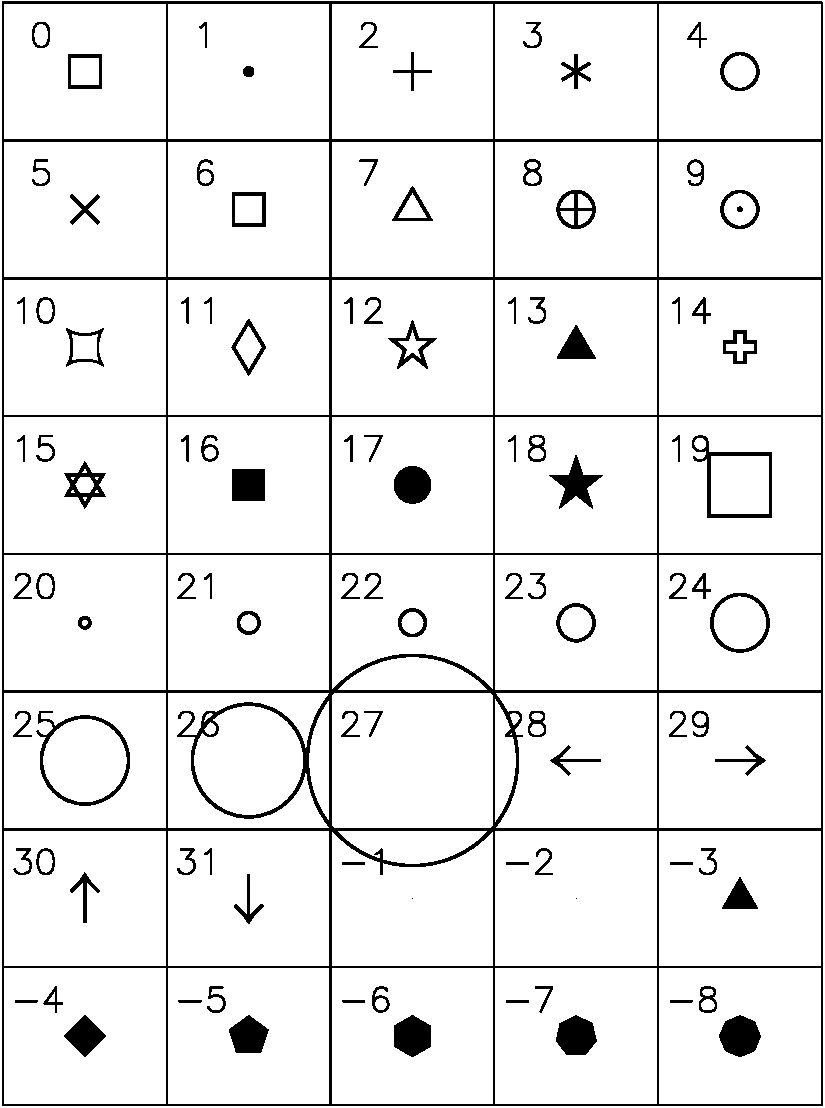
\includegraphics[width=5in]{plot-syms.pdf}
  \caption{Plotting Symbols.}
  \label{t:plot.syms}
\end{table}

The symbol types are:
\begin{example}
  square                 triangle                    square_concave              
  dot                    circle_plus                 diamond                     
  plus                   circle_dot                  star5                       
  times                  square_filled               triangle_filled           
  circle                 circle_filled               red_cross                 
  x                      star5_filled                star_of_david             
\end{example}
These symbols are illustrated in Table~\ref{t:plot.syms}. Symbol type names are case insensitive.

%-----------------------------------------------------------------
\subsection{qp_axis_struct}
\label{s:qp.axis}

The \vn{qp_axis_struct} structure defines the properties of a graph axis
\begin{example}
  type qp_axis_struct::
    label             = "<string>" ! Axis label string.
    min               = <real>     ! Min is the left or bottom axis number.
    max               = <real>     ! Max is the right or top axis number.
    number_offset     = <real>     ! Offset from axis line in inches.
    label_offset      = <real>     ! Offset from numbers in inches.
    major_tick_len    = <real>     ! Major tick length in inches.
    minor_tick_len    = <real>     ! Minor tick length in inches.
    label_color       = <string>   ! Color of the label string (\sref{s:qp.color})
    major_div         = <integer>  ! Number of major divisions
    major_div_nominal = <integer>  ! Major divisions nominal value.
    minor_div         = <integer>  ! Minor divisions. 0 = Tao will choose.
    minor_div_max     = <integer>  ! Max minor div number if Tao chooses.
    places            = <integer>  ! Number of digits to print
    type              = <string>   ! Axis type: "LINEAR" or "LOG".
    bounds            = <string>   ! Axis bounds: "GENERAL", "ZERO_AT_END", etc.
    tick_side         = <integer>  ! 1 = draw to the inside, 0 = both, -1 = outside.
    number_side       = <integer>  ! 1 = draw to the inside, -1 = outside.
    draw_label        = <logical>  ! Draw the label string
    draw_numbers      = <logical>  ! Draw the numbers.
\end{example}

The \vn{%bounds} parameter sets how the axes min and max values are calculated when plots are initially
instantiated and when \vn{scale}, \vn{x_scale}, and \vn{xy_scale} commands are used. Possible settings
are:
\begin{example}
  "ZERO_AT_END"      ! Min or max value is set to zero.
  "ZERO_SYMMETRIC"   ! Min and max chosen so that max = -min.
  "GENERAL"          ! No restrictions (default).
  "EXACT"            ! The User min/max is used.
\end{example}
If input min and max values are specified by the User, \tao will take the specified values as the starting
point to find ``nice'' min and max values to use. For example, with the command
\begin{example}
  scale all 0 19
\end{example}
and with \vn{bounds} set to \vn{"GENERAL"}, the min and max values will be set to 0 and 20. The exception is when
\vn{bounds} is set to \vn{"EXACT"}. In this case the User supplied min and max values will be used as is.

Examples:
\begin{example}
Tao> set graph r13 y%bounds = "zero_at_end"
Tao> scale r13 200 280   ! Graph bounds set to [0, 300]

Tao> set graph r13 y%bounds = "zero_symmetric"
Tao> scale r13 200 280   ! Graph bounds set to [-300, 300]

Tao> set graph r13 y%bounds = "general"
Tao> scale r13 20 190    ! Graph bounds set to [0, 200]

Tao> set graph r13 y2%bounds = "exact"
Tao> scale r13 -y2 20 190    ! Y2 graph bounds set to [20, 190]
\end{example}

Both \vn{major_div} and \vn{major_div_nominal} set the number of major divisions in the plot. The
difference between the two is that with \vn{major_div} set positive and \vn{major_div_nominal} set
zero or negative, the number of major divisions is fixed at the value of \vn{major_div}. With
\vn{major_div_nominal} positive, the value of \vn{major_div} is ignored, and the number of major
divisions will be chosen to be a ``nice'' value near the value of \vn{major_div_nominal}. If neither
\vn{major_div} nor \vn{major_div_nominal} is set positive, a value will be chosen for
\vn{major_div_nominal} by \tao. If you are unsure which to set, it is recommended that
\vn{major_div_nominal} be used.

The \vn{places} parameter set the number of places to display a number. \tao will automatically
calculate this number and it is not user settable.

The \vn{label} parameter may include Greek letters, subscripts, superscripts, and special characters.
Encoding for these are given in Table~\ref{t:plot.escape}. 


%-----------------------------------------------------------------
\subsection{String Escape Sequences}
\label{s:qp.str}

\begin{table}[tb]
\begin{tabular}{ll} \toprule
{\B}u       & Start a superscript or end a subscript \\[0.3ex]
{\B}d       & Start a subscript or end a superscript.
              {\B}u and {\B}d must always be used in pairs \\[0.3ex]
{\B}b       & Backspace (i.e., do not advance text pointer  
               after plotting the previous character) \\[0.3ex]
{\B}fn      & Switch to Normal font (1)       \\[0.3ex]
{\B}fr      & Switch to Roman font (2)        \\[0.3ex]
{\B}fi      & Switch to Italic font (3)       \\[0.3ex]
{\B}fs      & Switch to Script font (4)       \\[0.3ex]
{\B}{\B}    & Backslash character (\B)        \\[0.3ex]
{\B}x       & Multiplication sign ($\times$)  \\[0.3ex]
{\B}.       & Centered dot ($\cdot$)          \\[0.3ex]
{\B}A       & Angstrom symbol (\AA)         \\[0.3ex]
{\B}gx      & Greek letter corresponding to roman letter x. See Table~\ref{t:greek}. \\[0.3ex]
{\B}mN {\B}mNN & Graph marker number \vn{N} or \vn{NN} (1-31) \\[1ex]
{\B}(NNNN)  & 
\parbox{5.2in} {Character number NNNN (1 to 4 decimal digits) from the Hershey character set which
includes a number of special characters including mathematical, musical, astronomical, and
cartographical symbols.} \\ \bottomrule
\end{tabular}
\caption{Escape Sequences for Labels.}
\label{t:plot.escape}
\end{table}

Table~\ref{t:greek} shows how the character string \vn{"{\B}g<r>"}, where \vn{"<r>"} 
is a Roman letter, map onto the Greek character set.
\begin{table}[tb]
  \centering
  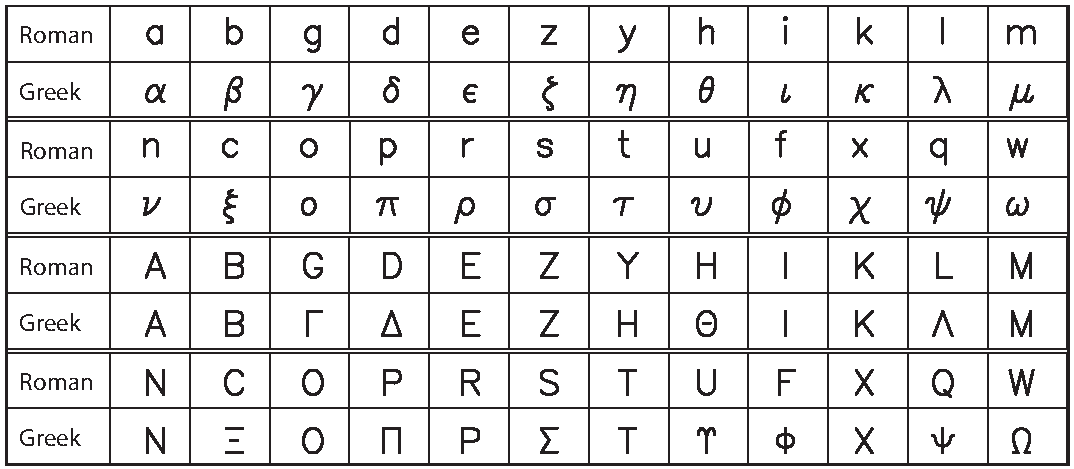
\includegraphics[width=5.0in]{greek.pdf}
  \caption[Roman to Greek Character Conversion]{Conversion for the string 
\vn{"{\B}g<r>"} where \vn{"<r>"} is a Roman character to the corresponding 
Greek character.}
\label{t:greek}
\end{table}

%-----------------------------------------------------------------
\subsection{Color Names}
\label{s:qp.color}

Possible settings for color parameters are:
\begin{example}
  White   (actually the background color)       Orange          
  Black   (actually the foreground color)       Yellow_Green    
  Red                                           Light_Green         
  Green                                         Navy_Blue       
  Blue                                          Purple          
  Cyan                                          Reddish_Purple  
  Magenta                                       Dark_Grey        
  Yellow                                        Light_Grey       
\end{example}
Color names are case insensitive.

%-----------------------------------------------------------------
\subsection{Line Pattern Names}
\label{s:qp.line.pat}

Possible settings for line patterns are:
\begin{example}
  solid      ! Solid line                 dotted     ! Dotted line             
  dashed     ! Dashed line                dash_dot3  ! Dash--dot--dot--dot line
  dash_dot   ! Dash--dot line
\end{example}
Pattern names are case insensitive.

%-----------------------------------------------------------------
\subsection{Fill Pattern Names}
\label{s:qp.fill.pat}

Possible fill pattern settings for symbols are:
\begin{example}
  solid_fill                    hatched           
  no_fill                       cross_hatched     
\end{example}
Fill pattern names are case insensitive.


\chapter{Data in Tao}
\label{c:data}
\index{data|hyperbf}

The term \vn{``data''} denotes anything that can be calculated by
\tao. This includes the vertical orbit at a particular position or the
horizontal emittance of a storage ring. Data can be plotted or used in
lattice correction and design (\sref{c:opti}). This chapter explains
how data is organized in \tao while Section~\sref{s:init.data}
explains how to define the structures that hold the data in the
initialization files. When running \tao, the \vn{show data}
(\sref{s:show}) command can be used to view information about the
data.


%------------------------------------------------------------------------
\section{Data Organization}
\label{s:data.org}

\begin{figure}
  \centering
  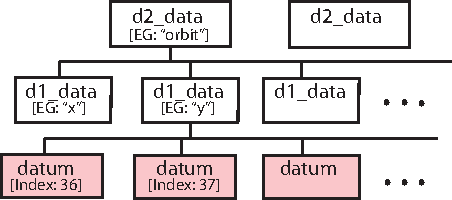
\includegraphics[width=4in]{data-tree.pdf}
  \caption[Data tree structure]
{A \vn{d2\_data} structure holds a set of \vn{d1\_data} structures. 
A \vn{d1\_data} structure holds an array of datums.}
  \label{f:data.tree}
\end{figure}

\index{d2_data}\index{d1_data}
The horizontal orbit at a particular BPM is an example of an
individual \vn{datum}.  For ease of manipulation, arrays of datums are
grouped into what is called a \vn{d1_data} structure. Furthermore,
sets of \vn{d1_data} structures are grouped into what is called a
\vn{d2_data} structure.  This is illustrated in
Figure~\ref{f:data.tree}.  For example, a \vn{d2_data} structure for
orbit data could contain two \vn{d1_data} structures --- one
\vn{d1_data} structure for the horizontal orbit data and another
\vn{d1_data} structure for the vertical orbit data. Each datum of,
say, the horizontal orbit \vn{d1_data} structure would then correspond
to the horizontal orbit at some point in the machine.

When issuing \tao commands, all the
data associated with a \vn{d2_data} structure is specified using the
\vn{d2_data} structure's \vn{name}.  The data associated with a
\vn{d1_data} structure is specified using the format
\begin{example}
  d2_name.d1_name
\end{example}
For example, if a \vn{d2_data} structure has the
name ``\vn{orbit}'', and one of its \vn{d1_data} structures has the
name ``\vn{x}'', then \tao commands that refer to the data in this
\vn{d1_data} structure use the name ``\vn{orbit.x}''. Sometimes there
is only one \vn{d1_data} structure for a given \vn{d2_data}
structure. In this case the data can be referred to simply by using
the \vn{d2_data} structure's name. The individual datums can be
referred to using the notation
\begin{example}
  <d2_name>.<d1_name>[<list_of_datum_indexes>]
\end{example}
For example, \vn{orbit.x[10]} refers to the horizontal orbit datum
with index 10. Notice that the beginning (lowest) datum index is user
selectable and is therefore not necessarily 1. 

It is important to note that the name given to \vn{d2_data} and \vn{d1_data}
structures is arbitrary and does not have to correspond to the 
type of data contained in the 
structures. In fact, a \vn{d1_data} array can contain heterogeneous data types.
Thus, for example, it is perfectly permissible (but definitely not recommended) 
to set up the data structures so that, say, \vn{orbit.x[10]} 
is the $a$-mode emittance at a certain element and \vn{orbit.x[11]}
is the $b$-mode beta function at the same element.

Ranges of data can be referred to using using a comma \vn{,} to
separate the indexes combined with the notation \vn{n1:n2} to specify
all the datums between \vn{n1} and \vn{n2} inclusive. For example
\begin{example}
  orbit.x[3:6,23]
\end{example}
refers to datums 3, 4, 5, 6, and 23. 

If multiple universes are present, then, as explained in
\sref{s:universe}, the prefix \vn{"@"} may be used to specify which
universe the data applies to. The general notation is
\begin{example}
  [<universe_range>]@<d2_name>.<d1_name>[<datum_index>]
\end{example}
Examples:
\begin{example}
  [2:4,7]@orbit.x ! The \vn{orbit.x} data in universes 2, 3, 4 and 7.
  [2]@orbit.x     ! The \vn{orbit.x} data in universe 2. 
  2@orbit.x       ! Same as "2@orbit.x".
  orbit.x         ! The \vn{orbit.x} data in the current viewed universe.
  -1@orbit.x      ! Same as "orbit.x".
\end{example}

As explained in Section~\sref{s:data.anatomy}, each individual datum
has a number of components. The syntax to refer to a component is:
\begin{example}
  d2_name.d1_name[datum_index]|component
\end{example}
For example:
\begin{example}
  orbit.x[3:10]|meas     ! The measured data values
\end{example}

In referring to datums, a ``\vn{*}'' can be used as a wild card to 
denote ``all''. Thus:
\begin{example}
  *@orbit.x       ! The \vn{orbit.x} data in all universes.
  *               ! All the data in the currently viewed universe.
  *.*             ! Same as "*"
  *@*             ! All the data in all the universes. 
  *@*.*           ! Same as "*@*"
  orbit.x[*]|meas ! All measured values of orbit.x
  orbit.x[]|meas  ! No values. That is, the empty set.
  orbit.x|meas    ! Same as orbit.x[*]|meas.
\end{example}
The last example shows that when referring to an entire block of data
encompassed by a \vn{d1_data} structure, the \vn{[*]} can be omitted.

%------------------------------------------------------------------------
\section{Anatomy of a Datum}
\label{s:data.anatomy}

Each datum has a number of quantities associated with it:
\begin{example}
  data_type        ! Character: Type of data: "orbit.x", etc.
  ele_name         ! Character: Name of lattice element where datum is evaluated.
  ele_start_name   ! Character: Name of starting lattice element in a range.
  ele_ref_name     ! Character: Name of reference lattice element.
  merit_type       ! Character: Type of constraint: "target", "max", etc.
  data_source      ! Character: How the datum is calculated. "lat", or "beam".
  ix_ele           ! Integer: Index of "ele" in the lattice element list.
  ix_ele_start     ! Integer: Index of "ele_start" in the lattice element list.
  ix_ele_ref       ! Integer: Index of "ele_ref" in the lattice element list.
  ix_ele_merit     ! Integer: Lattice index where merit is evaluated.
  ix_d1            ! Integer: Index number in d1_data structure
  ix_data          ! Integer: Index in the global data array
  ix_dModel        ! Integer: Row number in the dModel_dVar derivative matrix.
  ix_bunch         ! Integer: Bunch number to get the data from.
  meas             ! Real: Measured datum value. 
  ref              ! Real: Measured datum value from the reference data set.
  model            ! Real: Datum value as calculated from the model.
  design           ! Real: What the datum value is in the design lattice.
  old              ! Real: Used by \tao to save the model at some previous time.
  base             ! Real: The value as calculated from the base model.
  fit              ! Real: This value is not used by \tao.
  invalid          ! Real: The value used for delta_merit if good_model = False.
  delta_merit      ! Real: Diff used to calculate the merit function term 
  weight           ! Real: Weight for the merit function term
  merit            ! Real: Merit function term value: weight * delta^2
  s                ! Real: longitudinal position of ele.
  exists           ! Logical: Does the datum exist?
  good_model       ! Logical: Does the model  component contain a valid value?
  good_design      ! Logical: Does the design component contain a valid value?
  good_base        ! Logical: Does the base   component contain a valid value?
  good_meas        ! Logical: Does the meas   component contain a valid value?
  good_ref         ! Logical: Does the ref    component contain a valid value?
  good_user        ! Logical: Does the user want this datum used in optimization?
  good_opt         ! Logical: Can be used in Tao extensions.
  good_plot        ! Logical: Can be used in Tao extensions.
  useit_plot       ! Logical: Is this datum to be used in plotting?
  useit_opt        ! Logical: Is this datum to be used for optimization?
\end{example}
When running \tao, the \vn{show data}
(\sref{s:show}) command can be used to view the components of a datum. 
The \vn{set} command (\sref{s:set}) can be used to set some of these components.

%------------------------------------------------------------------------
\section{Datum values}
\label{s:datum.values}

\index{data!measured}\index{data!reference}\index{data!model}
\index{data!base}\index{data!design}
A given datum has six values associated it:
\vspace{-2ex}
\begin{description}
  \vspace{-1ex}
  \item[meas] \Newline 
The value of the datum as obtained from some measurement. This is the
target or limit value that is used when running the optimizer. When
doing lattice design, the measured value corresponds to a constraint
value (\ref{c:opti}).
  \vspace{-1ex}
  \item[base] \Newline
The datum value as calculated from the \vn{base} lattice (\sref{s:lattice}).
  \vspace{-0.5ex}
  \item[design] \Newline
The value of the datum as calculated from the \vn{design} lattice (\sref{s:lattice}).
  \vspace{-0.5ex}
  \item[fit] \Newline
The \vn{fit} value is not used by \tao directly and is available for use by custom code.
  \vspace{-0.5ex}
  \item[model] \Newline
The value of the datum as calculated from the \vn{model} lattice (\sref{s:lattice}).
  \vspace{-0.5ex}
  \item[old] \Newline
A datum value that was saved at some point in \tao's calculations. This value
can be ignored.
  \vspace{-0.5ex}
  \item[ref] \Newline
The reference datum value as obtained from some reference measurement. For example,
a measurement before some variable is varied could be designated as
the \vn{reference}, and the datum taken after the variation could be 
designated the \vn{measured} datum.
\end{description}

%------------------------------------------------------------------------
\section{Datums in Optimization}
\label{s:datum.opt}

When using optimization for lattice correction or lattice design
(\sref{c:opti}), Individual datums can be excluded from the process
using the \vn{veto} (\sref{s:veto}), \vn{restore} (\sref{s:restore}),
and \vn{use} (\sref{s:use}) commands. These set the \vn{good_user}
component of a datum. This, combined with the setting \vn{exists},
\vn{good_meas}, \vn{good_ref}, and \vn{good_opt}
determine the setting of \vn{useit_opt} which is the component that
determines if the datum is used in the computation of the merit
function. The settings of everything but \vn{good_user} is determined
by \tao

The \vn{exists} component is set by \tao to True if the datum exists
and False otherwise. A datum may not exist if the type of datum
requires the designation of an associated element but the
\vn{ele_name} component is blank. For example, a \vn{d1_data} array
set up to hold orbit data may use a numbering scheme that fits the
lattice so that , say, datum number 34 in the array does not
correspond to an existing BPM.

The \vn{good_model} component is set according to whether a datum
value can be computed from the \vn{model} lattice. For example, If a
circular lattice is unstable, the beta function and the closed orbit
cannot be computed. Similarly, the \vn{good_design} and \vn{good_base}
components mark whether the \vn{design} and \vn{base} values
respectively are valid.

When doing optimization, the \vn{delta_merit} component is set to the
\vn{delta} value used in computing the contribution to the merit
function (\sref{s:generalized.design}). If the datum's value cannot be
computed, that is, \vn{good_model} is False, or, if the design or base
values are being used in the merit calculation, \vn{good_base} or
\vn{good_design} is False, then the \vn{invalid} component is used for
\vn{delta_merit}.

\vn{good_meas} is set True if the \vn{meas} component value is set in
the data initialization file (\sref{s:init.data}) or is set using the
\vn{set} command (\sref{s:set}). Similarly, \vn{good_ref} is set True
if the \vn{ref} component has been set. \vn{good_ref} only affects the
setting of \vn{useit_opt} if the optimization is using reference data
as set by the global variable \vn{opt_with_ref} (\sref{s:globals}).

Finally \vn{good_opt} is meant for use in custom versions of \tao
(\sref{c:custom.tao}) and is always left True by the standard \tao code.

Example of using a \vn{show data} (\sref{s:show}) to check the logicals
in a datum:
\begin{example}
  Tao> show data 3@beta[1]

  Universe:   3
  %ele_name          = IP_L0
  %ele_ref_name      =
  %ele_start_name    =
  %data_type         = beta.a
      ... etc ...
  %exists            =  T
  %good_model        =  T
  %good_meas         =  F
  %good_ref          =  F
  %good_user         =  T
  %good_opt          =  T
  %good_plot         =  F
  %useit_plot        =  F
  %useit_opt         =  F
\end{example}
Here \vn{useit_opt} is False since \vn{good_meas} is False and
\vn{good_meas} is False since the \vn{meas} value of the datum (not
shown) was not set in the \tao initialization file.

%------------------------------------------------------------------------
\section{Data_source}
\index{data!data_source}
\label{s:data.source}

The \vn{data_source} component specifies where the data is 
coming from. Possible values are:
\begin{example}
  "beam"      ! Calculation using the beam distribution.
  "lat"       ! Calculation using the lattice.
\end{example}
If \vn{data_source} is set to \vn{"beam"}, the data is calculated
using multiparticle tracking.  If \vn{data_source} is set to
\vn{"lat"}, the data is calculated using the ``lattice'' which here
means everything {\em but} multiparticle tracking.  For example, the
\vn{"beam"} based calculation of the emittance uses the bunch sigma
matrix obtained through multiparticle tracking. The \vn{"lat"} based
calculation of the emittance uses radiation integrals.

Some data types may be restricted as to which \vn{data_source} is
possible. For example, a datum with \vn{data_type} set to
\vn{n_particle_loss} must use \vn{"beam"} for the \vn{data_source}. 
Table~\ref{t:data.types} lists which \vn{data_source} values are valid
for what data types.

%------------------------------------------------------------------------
\section{Datum Evaluation and Associated Lattice Elements}
\index{data!associated lattice elements}
\label{s:data.lat.ele}

Datums can be divided up into two classes. In one class are the datums
that are \vn{``local''}, like the beam orbit, which need to be evaluated at
either a particular point are evaluated over some finite region of the
machine. Other datums, like the emittance, are \vn{``global''} and do not
have associated evaluation points.

As mentioned, \vn{local} datums may be evaluated at a specific point
or over some evaluation region, an evaluation region is used when, for
example, the maximum or minimum value over a region is wanted. To
specify an evaluation point, an \vn{evaluation element} must be
associated with a datum. The evaluation point will be at the exit end
of this element. To specify an evaluation region, a \vn{start element}
must also be associated with a datum along with the \vn{evaluation
element}. The evaluation region is from the exit end of the \vn{start
element} to the exit end of the \vn{evaluation element}.

In addition to the \vn{evaluation element} and the \vn{start element},
a \vn{local} datum may have an associated \vn{reference element}.  A
\vn{reference element} is used as a fiducial point and the datum value
is calculated relative to that point. For example, a datum value may
be the position of the \vn{evaluation element} relative to the
position of the \vn{reference element}. The evaluation point of a
\vn{reference element} is the exit end of that element.

The components in a datum corresponding to the \vn{evaluation
element}, the \vn{reference element}, and the \vn{start element}.  are
shown in Table~\ref{t:datum.elements}.  These three elements may be
specified for a datum by either setting the name component or the
index component of the datum. Using the element index over the element
name is necessary when more than one element in the lattice has the
same name.

\begin{table}[htb]
\centering
\begin{tabular}{lll}
  \toprule
  &\multicolumn{2}{c}{\it Data Component} \\ \cmidrule{2-3}
  {\it Element} & {\it name} & {\it index} \\ \midrule
  Reference Element  & \vn{ele_ref_name}   & \vn{ix_ele_ref}   \\
  Start Element      & \vn{ele_start_name} & \vn{ix_ele_start} \\
  Evaluation Element & \vn{ele_name}       & \vn{ix_ele}       \\ \bottomrule
\end{tabular}
\caption[The three lattice elements associated with a datum.]
{The three lattice elements associated with a datum may be
specified in the datum by setting the appropriate name component or by 
setting the appropriate index component.}
\label{t:datum.elements}
\end{table}

If a datum has an associated \vn{evaluation} element, but no
associated \vn{start} or \vn{reference} elements, the \vn{model} value
of that datum is the value of the \vn{data_type} at the \vn{evaluation}
element. For example, if a datum has:
\begin{example}
  data_type      = "orbit.x"
  ele_name       = "q12"
\end{example}
here the \vn{model} value of this datum will be the horizontal orbit
at the element with name \vn{q12}.

If a datum has an associated \vn{start} element, specified by either
setting the \vn{ele_start_name} or \vn{ix_ele_start} datum components, the
datum is evaluated over a region from the exit end of the \vn{start} element
to the exit end of \vn{evaluation} element. For example, if a datum has:
\begin{example}
  data_type      = "beta.a"
  ele_name       = "q12"
  ele_start_name = "q45"
  merit_type     = "max"
\end{example}
then the \vn{model} value of this datum will be the maximum value of
the a-mode beta function in the region from the exit end of the
element with name \vn{q12} to the exit end of the element with name
\vn{q45}. Notice that when a range of elements is used, a
\vn{merit_type} of \vn{target} does not make sense. 

Typically, in evaluating a datum over some region to find the maximum
or minimum, \tao will only evaluate the datum at the ends of the
elements with the assumption that this is good enough. If this is not
good enough, marker elements can be inserted into the lattice at
locations that matter. For example, the maximum or minimum of the beta
function typically occurs near the middle of a quadrupole so inserting
marker elements in the middle of quadrupoles will improve the accuracy
of finding the extremum beta.

If a datum has an associated \vn{reference} element, specified by either
setting the \vn{ele_ref_name} or \vn{ix_ele_ref} datum components, the
\vn{model} value of the datum is the value at the \vn{evaluation} element (or the value
over the range \vn{ele_start} to the \vn{evaluation} element if \vn{ele_start} is
specified), minus the \vn{model} value at \vn{ele_ref}. For example,
if a datum has:
\begin{example}
  data_type      = "beta.a"
  ele_name       = "q12"
  ele_start_name = "q45"
  ele_ref_name   = "q1"
  merit_type     = "max"
\end{example}
then the \vn{model} value of the datum will be the same as the
previous example minus the value of the a-mode beta function at the
exit end of element \vn{q1}. There are a number of exceptions to the
above rule and datum types treat the \vn{reference} element in a different
manner. For example, the \vn{r.} data type uses the \vn{reference} element
as the starting point in constructing a transfer matrix.

%------------------------------------------------------------------------
\section{Tao Data Types}\index{data!data Types}
\label{s:data.types}

The \vn{data_type} component of datum specifies what type of data the
datum represents. For example, a datum with a \vn{data_type} of
\vn{orbit.x} represents the horizontal orbit. Table~\ref{t:data.types} lists
what data types \tao knows about.

It is important to note the difference between the \vn{d2.d1} name
that is used to refer to a datum and the actual type of data, given by
\vn{data_type}, of the datum. The \vn{d2.d1} name is arbitrary and is
specified in the \tao initialization file (\sref{s:init.data}). Often,
these names do reflect the actual type of data. However, there is no
mandated relationship between the two. For example, it is perfectly
possible to set create a data set with a \vn{d2.d1} name of
\vn{orbit.x} to hold, say, global floor position data. In fact, the
datums in a given \vn{d1} array do not all have to be of the same
type. Thus the user is free to group data as s/he sees fit.

Description of the data types:

  \begin{description}
  \index{apparent_emit.}
  \item[apparent_emit.] \Newline
The apparent emittance is the emittance that one would calculate based
upon a measurement of the beam size\cite{b:emit}. It can be useful to
compare this to the true normal mode emittance. Also See the
\vn{norm_apparent_emit}, \vn{emit.} and \vn{norm_emit.} data types.
With \vn{data_source} set to \vn{"beam"}, \vn{apparent_emit.x} is
\begin{equation}
  E_x = \frac{\sigma_{xx} - \eta_x^2 \, \sigma_{p_zp_z}}{\beta_a}
\end{equation}
with a similar equation for \vn{apparent_emit.y}. Here $\sigma$ is the beam size matrix
\begin{equation}
  \sigma_{r_1r_2} \equiv \left< r_1 \, r_2 \right>
\end{equation}
With \vn{data_source} set to \vn{"lat"}, The apparent emittance is
calculated from the true normal mode emittance and the Twiss
parameters (Cf.~ Eqs (4) and (5) of \cite{b:emit}).

  \index{beta.}
  \item[beta.] \Newline
\vn{beta.a} and \vn{beta.b} are the lattice beta functions. \vn{beta.x} and
\vn{beta.y} are beam projected beta functions defined by
\begin{equation}
  \beta.x = \frac{<x^{2}>}{\sqrt{<x^{2}> <x'^{2}> - <x x'>^{2}}}.
\end{equation}
where the average \vn{<>} is over all the particles in the beam.

Note: If the beta function is calculated from the beam distribution,
the emittance must be non-zero.

  \index{element_attrib.}
  \item{element_attrib.} \Newline
The \vn{element_attrib.<attrib_name>} data type is associated with the
lattice element attribute named \vn{<attrib_name>}. For any given
element, if \vn{<attrib_name} is not associated with the element, the
value of the datum is zero.

  \index{emit.}
  \item[emit.] \Newline
The \vn{emit.} data type covers two types of
``emittance''. \vn{emit.a}, \vn{emit.b}, and \vn{emit.c} are the true
normal mode (eigen) emittances. \vn{emit.x}, \vn{emit.y}, and
\vn{emit.z} are the ``projected'' emittances\cite{b:emit}. 
For a linear lattice, the emittance varies along the length
of the line while for a circular lattice there is a single emittance
number. 

With \vn{data_source} set to \vn{"beam"}, the emittance is calculated
from the beam sigma matrix. For the eigen emittance this involves the
standard normal mode decomposition. For the projected emittance, the
formula for $\epsilon_x$ is
\begin{equation}
  \epsilon_x = \sqrt{ \wt\sigma_{xx} \, \wt\sigma_{p_xp_x} - \wt\sigma_{xp_x}^2}
\end{equation}
With a similar equation for $\epsilon_y$. Here $\wt\sigma$ is the energy normalized
beam size:
\begin{equation}
  \wt\sigma_{xx} = \langle x \, x \rangle - 
  \frac{\langle x \, p_z \rangle \, \langle x \, p_z \rangle}{\langle p_z \, p_z \rangle}
\end{equation}
with similar definitions for the other $\wt\sigma$ components. 
Note that the projected emittance is sometimes defined using
$x'$ and $y'$ in place of $p_x$ and $p_y$. However, in the vast
majority of cases, this does not appreciably affect the numeric
results.

With \vn{data_source} set to \vn{"lat"}, the normal mode emittance is calculated
using the standard radiation integrals.

See also the \vn{norm_emit.}, \vn{apparent_emit.}, and
\vn{norm_apparent_emit.} data types.

  \index{expression: }
  \item[expression:] \Newline
The \vn{expression:} The data type can be an expression (\sref{s:arithmetic.exp}).
In this case the \vn{data_type} must begin with the string ``\vn{expression:}''.
For example:
\begin{example}
  datum(i)%data_type = "expression: 1@lat::q10w[beta_a] - 2@lat::q10w[beta_a]"
\end{example}
With this, the value of the datum will be the difference between
the a-mode beta at element \vn{q10w}
for universe 1 and universe 2. In this example,
the source of both terms in the expression is explicitly given as \vn{lat}.
This is not necessary if the \vn{datum%data_source} is set to \vn{lat}
\begin{example}
  datum(i)%data_type = "expression: 1@q10w[beta_a] - 2@q10w[beta_a]"
  datum(i)%data_source = "lat"
\end{example}
An expression can also be used as the
\vn{default_data_type}. In this case, the 
evaluation point is implicit. For example:
\begin{example}
  default_data_source = "dat"
  default_data_type = "expression: 1@beta.a - 2@beta.a"
\end{example}
which is equivalent to:
\begin{example}
  default_data_type = "expression: 1@dat::beta.a - 2@dat::beta.a"
\end{example}

To be valid, if an expression has a term with a \vn{dat} source, the
expression must be evaluated after the \vn{dat} source components are
evaluated. Data evaluation is done universe by universe starting with
universe 1, then universe 2, etc. Within a given universe, the order
of evaluation can be complicated but in this case a datum using an
expression will always be evaluated after any datum that appears
earlier in the initialization file.  In the last example above, the
expression terms involve an evaluation of \vn{beta.a} in universe 2.  
Therefore, this expression datum should
be in universe 2 or higher. Notice that while all datums must be
assigned a universe, in this case, since all the terms explicitly give
a universe number, the value of the datum will be independent of the
universe it is in.

  \index{floor.}
  \item[floor.] \Newline
This is the global floor position at the exit end of evaluation element. See the
\bmad manual for details on the global coordinate system. See also
\vn{rel_floor.}.

  \index{n_particle_loss}
  \item[n\_particle\_loss] \Newline
If the reference element is not specified, \vn{n_particle_loss} gives
the number of particles lost at the evaluation element. If the
reference element is specified, \vn{n_particle_loss} gives the
cumulative loss between the exit end of the reference element and the
exit end of the evaluation element. That is, this sum does not count
any losses at the reference element itself. If neither reference nor
evaluation element is given then the total number of lost particles is
given.

  \index{norm_apparent_emit.}
  \item[norm_apparent_emit.] \Newline
The \vn{norm_apparent_emit.} data type is the energy normalized
apparent emittance. The normalization is the standard gamma factor:
\Begineq
  E_{norm} = \gamma \, E
\Endeq
See the \vn{apparent_emit.} data type for more details.

  \index{norm_emit.}
  \item[norm_emit.] \Newline
The \vn{norm_emit.} data type is the energy normalized
emittance. The normalization is the standard gamma factor:
\Begineq
  \epsilon_{norm} = \gamma \, \epsilon
\Endeq
See the \vn{apparent_emit.} data type for more details.


  \index{periodic.tt.}
  \item[periodic.tt.] \Newline
This is like the \vn{tt.} datum except here the terms are from the
periodic Taylor map defined by
\Begineq
  T_p \equiv (T_0 - I_4)^{-1}
\Endeq
Here $T_p$ is the
periodic map, $T_0$ is the one-turn map from some point back to that
point, and $I_4$ is a linear map defined by the matrix
\Begineq
  I_4 \equiv 
    \begin{pmatrix}
      1 &   &   &   &   &   \\
        & 1 &   &   &   &   \\
        &   & 1 &   &   &   \\
        &   &   & 1 &   &   \\
        &   &   &   & 0 &   \\
        &   &   &   &   & 0
    \end{pmatrix}
\Endeq
The periodic map give information about the closed orbit, dispersion,
etc. For example, the zeroth order terms are the closed orbit, the r16
term gives the horizontal dispersion, etc.

If a reference lattice element is specified, the map $T_0$ will be
the transfer map from the reference element to the evaluation element.

Note: If the reference element is not specified, or if the reference
element is the same as the evaluation element, this data type cannot
be used with a linear lattice.

  \index{phase.}
  \item[phase.] \Newline
This is the betatron phase.  If a \vn{d1_data} array has a set of
\vn{phase} datums, and if the reference element is {\em not}
specified, the average phase used for optimizations ($D$ in
\Eq{miwdjw}) and plotting for all the datums within a \vn{d1_data}
array are set to zero by adding a fixed constant to all the datums.
This is done since, without a reference point that defines a zero
phase, the overall average phase is arbitrary and so the average phase
is taken in \tao to be zero. This can be helpful in optimizations
since one does not have to worry about arbitrary offsets between the
\vn{model} and \vn{measured} values. If the reference element is
specified then there is no arbitrary constant in the evaluation.

  \index{rad_int.}
  \item[rad_int, rad_int1] \Newline
The \vn{rad_int.} datums are the radiation integrals from the start of
the lattice. The \vn{rad_int1.} datums are the radiation integrals on
an element-by-element basis. That is, if \vn{ele_ref} is not specified,
\vn{rad_int.} will give the radiation integral from the start of the 
lattice through the evaluation element, and \vn{rad_int1.} will give
the radiation integral integrated over just the evaluation element.

  \index{ref_time}
  \item[ref_time] \Newline
This is the time the reference particle passes the exit end of the element.
If the particle is ultra-relativistic then this is just $c * s$ where $s$
is the longitudinal distance from the start of the lattice.

  \index{rel_floor.}
  \item[rel\_floor.] \Newline
This is the global floor position at the exit end of the evaluation
element relative to the exit end of the reference element in a global
coordinate system where the exit end of the reference element is taken to be at
\vn{x = y = z = theta = phi = 0}. See the \bmad manual for details on
the global coordinate system. See also \vn{floor.}.

  \index{t. tt.} 
  \item[t. tt.] \Newline
The \vn{t} and \vn{tt} data types give terms of the Taylor map between
two points. The difference between \vn{t.} and \vn{tt.} is that
\vn{t.} is restricted to exactly three indices and \vn{tt.} is
not. \vn{t.} is superfluous but is keep for backwards compatibility.

Calculation of \vn{t.} and \vn{tt.} datums involve symplectic
integration through lattice elements. One point to be kept in mind is
that results will be dependent upon the integration step size through
an element set by the \vn{ds_step} attribute of that element (see the
\bmad manual for more details). When a smooth curve
(\sref{s:template}) is plotted for \vn{t} and \vn{tt} data types, and
the longitudinal (\vn{"s"}) position is used for the x-axis, the
integration step used in generating the points that define this curve
will be decreased if the s-distance between points is smaller than
the \vn{ds_step}.  In this case, discrepancies between the plot and
datum values may be observed.

  \index{unstable.orbit}
  \item[unstable.orbit] \Newline
The \vn{unstable.orbit} datum is used for linear lattices in an
optimization to avoid unstable solutions (\sref{s:generalized.design}).

For single particle tracking, the value of an \vn{unstable.orbit}
datum is zero if the tracked particle survives (has not been lost) up
to the evaluation element and, if it has been lost, is set to
\Begineq
 1 + i_{\mbox{ele}} - i_{\mbox{lost}} + \frac{1}{2}
 \left[ \tanh\left( \frac{r_{orbit}}{r_{lim}} - 1 \right) - E \right]
\Endeq
where $i_{\mbox{ele}}$ is the index of the evaluation element in the
lattice and $i_{\mbox{lost}}$ is the index of the element where the
particle was lost. In the above equation, $E$ is the function
\Begineq
  E = 
  \begin{cases}
    1 & \text{if the particle is lost at the exit end of the element.} \\
    0 & \text{if the particle is lost at the entrance end of the element.}
  \end{cases}
\Endeq
In the abouve equation, $r_{orbit}$ is the particle amplitude at the
point of loss and $r_{lim}$ is the aperture limit. The form of the
above equation has been choisen so that the datum value will be
monotonic with increasing stability.

The default for the evaluation element, if \vn{ele_name} nor
\vn{ix_ele} is not specified, is to use the last element in the
lattice. 

When tracking beams, the value of \vn{unstable.orbit} is the averaged
value over all particles in the bunch.

  \index{unstable.ring}
  \item[unstable.ring] \Newline
\vn{unstable.ring} is used for storage rings. The value of an
\vn{unstable.ring} datum is zero if the ring is stable and set to the
largest growth rate of all the normal modes of oscillation if the ring
is unstable. \vn{unstable.ring} is used in an optimization to avoid
unstable solutions (\sref{s:generalized.design}).

\begin{figure}
  \centering
  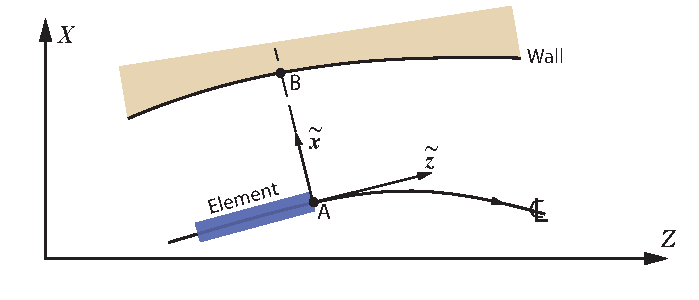
\includegraphics[width=5in]{building-wall-constraint.pdf}
  \caption[Building wall datum]
{A \vn{wall.} datum is a measure of the distance between the
centerline of a machine and the walls of the containment building.}
  \label{f:wall.constraint}
\end{figure}

  \index{wall.}
  \item[wall.] \Newline
The \vn{wall.} data types are used to constrain the shape of a machine
to fit inside a building's walls (\sref{s:building.wall}). The general
layout is shown in Figure~\ref{f:wall.constraint}. The machine
centerline is projected onto the horizontal $(Z, X)$ plane in the
Global (floor) coordinate system. Point \vn{A} is an evaluation point
at the exit end of some element. $\wt z$ is the projection of the
local $z$-axis onto the $(Z, X)$ plane and $\wt x$ is the coordinate
in the $(Z, X)$ plane perpendicular to $\wt z$. In the typical
situation, where a machine is planer (no out-of-plane bends), the $\wt
z$-axis corresponds to the local $z$-axis and the $\wt x$-axis
corresponds to the $x$-axis (see the \bmad manual for an explanation
of local and global coordinate systems).

The distance from the machine at point \vn{A} to the wall is defined
to be the distance from \vn{A} to a point \vn{B} on the wall where
point \vn{B} is along the $\wt x$ axis (has $\wt z = 0$) as shown in
Figure~\ref{f:wall.constraint}.

By definition, the \vn{``left side''} of the machine corresponds to be
the $+\wt x$ side and the \vn{``right side''} corresponds to be the
$-\wt x$ side. That is, left and right are relative to someone looking
in the same direction as the beam is propagating. Correspondingly,
there are two wall data types: \vn{wall.left_side} and
\vn{wall.right_side}. With the \vn{wall.left_side} data type, the
datum value is positive if point \vn{B} is on the left side and
negative if on the right. Vice versa for a \vn{wall.right_side} datum.
If there are multiple wall points \vn{B}, that is, if there are
multiple points on the wall with $\wt z = 0$, the datum value will be
the minimum value. Notice that only wall sections that have a
\vn{constraint} matching the datum will be used when searching for
possible points \vn{B}. If there are no wall points with $\wt z = 0$,
the datum value is set to a large number.

For \vn{wall} data there can be no reference element since this does
not make sense.

  \index{wire.}
  \item[wire] \Newline
\vn{wire} data simulates the measurement of a wire scanner. The angle
specified is the angle of the wire with respect to the horizontal
axis. The measurement then measures the second moment $<uu>$ along an
axis which is 90 degrees off of the wire axis. For example,
\vn{wire.90} is a wire scanner oriented in the vertical direction and
measures the second moment of the beam along the horizontal axis,
$<xx>$. The resultant data is not the beam size, but the beam size
squared.

  \end{description}


\index{data!calculation method}
\index{unstable.orbit}\index{beta}\index{alpha}\index{eta}\index{eta}
\index{etap}\index{phase}\index{orbit}\index{wire}\index{building wall}\index{spin}
\index{cbar}\index{coupling}\index{floor}\index{r}\index{t}\index{tt}
\index{rad_int.i5a_e6}\index{rad_int.i5b_e6}\index{s_position}\index{e_tot}
\index{unstable.ring}\index{emittance}\index{chrom}\index{norm_emittance}
\index{sigma}\index{dpx_dx}\index{dpy_dy}\index{dpz_dz}\index{dpa_da}
\index{dpb_db}\index{rad_int.i1}\index{rad_int.i2}\index{rad_int.i2_e4}
\index{rad_int.i3}\index{rad_int.i3_e7}

%----------------------------------------------------------------------------------------------

{\tt\small
\begin{longtable}{lll} 
  \caption{Predefined Data Types in Tao}
  \label{t:data.types}
  \\ \hline

  {\it Data\_Type}                    & {\it Description}                             & Source    \\ \hline\hline 
  \endfirsthead

  \caption[]{(continued)} \\ \hline
  {\it Data\_Type}                    & {\it Description}                             & source    \\ \hline\hline 
  \endhead

  alpha.a, alpha.b                    & Normal-Mode alpha function                    & lat       \\ \hline 
  apparent\_emit.x, apparent\_emit.y  & Apparent emittance                            & beam, lat \\ \hline
  beta.a, beta.b, beta.c              & Normal-mode beta function                     & beam, lat \\ \hline 
  beta.x, beta.y  beta.z              & Projected beta function                       & beam, lat \\ \hline 
  bpm\_orbit.x, bpm\_orbit.y          & Measured orbit                                & lat       \\ \hline
  bpm\_phase.a, bpm\_phase.b          & Measured betatron phase                       & lat       \\ \hline
  bpm\_eta.x, bpm\_eta.y              & Measured dispersion                           & lat       \\ \hline

  \begin{tabular}{@{}l}
    bpm\_k.22a, bpm\_k.12a, \\
    bpm\_k.11b, bpm\_k.12b
  \end{tabular}                       & Measured coupling                             & lat       \\ \hline

  \begin{tabular}{@{}l}
    bpm\_cbar.22a, bpm\_cbar.12a, \\
    bpm\_cbar.11b, bpm\_cbar.12b
  \end{tabular}
                                      & Measured coupling                             & lat       \\ \hline

  cbar.11, cbar.12, cbar.21, cbar.22
                                      & Coupling                                      & lat       \\ \hline 

  chrom.a, chrom.b                    & Chromaticity for a ring                       & lat       \\ \hline

  dpx\_dx, dpx\_dy, etc.              & Bunch <x px> / <$x^2$> \& Etc...              & beam      \\ \hline 

  e\_tot                              & Beam total energy (eV)                        & lat       \\ \hline

  element\_attrib.<attrib\_name>      & lattice element attribute                     & lat       \\ \hline

  emit.a, emit.b, emit.c              & Emittance                                     & beam, lat \\ \hline

  eta.x, eta.y, eta.z                 & Lab Frame dispersion                          & beam, lat \\ \hline 
  eta.a, eta.b                        & Normal-mode dispersion                        & beam, lat \\ \hline 
  etap.x, etap.y                      & Lab Frame dispersion derivative               & beam, lat \\ \hline 
  etap.a, etap.b                      & Normal-mode dispersion derivative             & beam, lat \\ \hline 

  expression: <arithmetic expression> & See the text                                  & lat       \\ \hline 

  floor.x, floor.y, floor.z, floor.theta 
                                      & Global (``floor'') position                   & lat       \\ \hline 

  gamma.a, gamma.b                    & Normal-mode gamma function                    & lat       \\ \hline 

  rad\_int.i1                         & I1 radiation integral                         & lat       \\ \hline
  rad\_int.i2                         & I2 radiation integral                         & lat       \\ \hline
  rad\_int.i2\_e4                     & Energy normalized I2 radiation integral       & lat       \\ \hline
  rad\_int.i3                         & I3 radiation integral                         & lat       \\ \hline
  rad\_int.i3\_e7                     & Energy normalized I3 radiation integral       & lat       \\ \hline
  rad\_int.i5a, rad\_int.i5b          & I5 radiation integrals                        & lat       \\ \hline
  rad\_int.i5a\_e6, rad\_int.i5b\_e6  & Energy normalized I5 radiation integral       & lat       \\ \hline

  k.11b, k.12a, k.12b, k.22a          & Coupling                                      & lat       \\ \hline 
  momentum                            & Momentum: P*C\_light (eV)                     & lat       \\ \hline
  momentum\_compaction                & Momentum compaction factor                    & lat       \\ \hline

  \begin{tabular}{@{}l}   
    multi\_turn\_orbit.x, multi\_turn\_orbit.px \\ 
    multi\_turn\_orbit.y, multi\_turn\_orbit.py \\
    multi\_turn\_orbit.z, multi\_turn\_orbit.pz \\
  \end{tabular}                       & Bunch size                                    & lat       \\ \hline 

  n\_particle\_loss                   & Number of particles lost                      & beam      \\ \hline 

  \begin{tabular}{@{}l}
    norm\_apparent\_emit.x \\
    norm\_apparent\_emit.y 
  \end{tabular}                       & Normalized apparent emittance                 & beam, lat \\ \hline
  norm\_emit.a, norm\_emit.b, norm\_emit.c 
                                      & Normalized beam emittance                     & beam, lat \\ \hline 
  norm\_emit.x, norm\_emit.y, norm\_emit.z
                                      & Energy Normalized projected emittance         & beam, lat \\ \hline 

  orbit.x, orbit.y, orbit.z           & Orbit                                         & beam, lat \\ \hline 
  orbit.px, orbit.py, orbit.pz       & Momenta                                       & beam, lat \\ \hline 
  orbit.amp\_a, orbit.amp\_b          & ``Invariant'' amplitude                       & lat       \\ \hline 
  orbit.norm\_amp\_a, orbit.norm\_amp\_b  
                                      & Energy normalized ``invariant'' amplitude     & lat       \\ \hline 

  periodic.tt.$ijklm\ldots$ \hspace{10pt} $1 \le i,j,k,\ldots \le 6$   
                                      & Taylor term of the periodic map.              & lat       \\ \hline 

  phase.a, phase.b                    & Betatron phase                                & lat       \\ \hline 

  phase\_frac.a, phase\_frac.b        & \begin{tabular}{@{}l}
                                         Fractional betatron phase \\       
                                         $-\pi < \phi_{\mbox{frac}} < \pi$ \\
                                       \end{tabular}                                 & lat        \\ \hline 

  phase\_frac\_diff                   & \begin{tabular}{@{}l}
                                         Fractional betatron phase \\
                                        difference (a-b) $-\pi < d\phi_{\mbox{frac}} < \pi$
                                       \end{tabular}                                 & lat       \\ \hline 

  photon.intensity_x, photon.intensity_y
                                      & Photon intensity                              & beam, lat \\ \hline
  photon.intensity                    & Photon total intensity                        & beam, lat \\ \hline 
  photon.phase_x, photon.phase_y      & Photon phase                                  & beam, lat \\ \hline

  r.$ij$ \hspace{10pt} $1 \le i,j \le 6$
                                      & Term in linear transfer map                   & lat       \\ \hline 

  ref\_time                           & Reference time                                & beam, lat \\ \hline

  \begin{tabular}{@{}l}   
    rel\_floor.x, rel\_floor.y, \\
    rel\_floor.z, rel\_floor.theta \\
  \end{tabular}                       & Relative global (``floor'') position          & lat       \\ \hline 

  s\_position                         & longitudinal length constraint                & lat       \\ \hline 

  \begin{tabular}{@{}l}   
    sigma.x, sigma.y, sigma.z \\ 
    sigma.px, sigma.py, sigma.pz
  \end{tabular}                       & Bunch size                                    & beam, lat \\ \hline 

  spin.polarization, spin.theta, spin.phi
                                      & Particle spin                                 & beam, lat \\ \hline 
  time                                & Particle time (sec)                           & lat       \\ \hline
  t.$ijk$ \hspace{10pt} $1 \le i,j,k \le 6$
                                      & Term in 2\Nd order transfer map               & lat       \\ \hline 
  tt.$ijklm\ldots$ \hspace{10pt} $1 \le i,j,k,\ldots \le 6$
                                      & Term in n\Th order transfer map               & lat       \\ \hline 

  tune.a, tune.b                      & Tune                                          & lat       \\ \hline 
  unstable.orbit                      & Nonzero if particles are lost in tracking     & lat       \\ \hline
  unstable.ring                       & Nonzero if a ring is unstable                 & lat       \\ \hline
  wire.<angle>                        & Wire scanner at wire angle <angle>            & beam      \\ \hline
  wall.left\_side, wall.right\_side   & Building wall constraint                      & lat       \\ \hline
\end{longtable}
}

\chapter{Variables}
\label{c:var}
\index{variables}

\index{change command}
\index{optimizer!variables}
For the \vn{model} lattice (or lattices if there are multiple \vn{universes}) the
\vn{change} command (\sref{s:change}) can be used to vary lattice parameters such as
element strengths, the initial Twiss parameters, etc.  Additionally, \vn{variables} can be
defined in the \tao initialization files (\sref{s:init.var}) that can also be used to vary
these \vn{model} lattice parameters.  A given \tao variable may control a single attribute
of one element in one or more universes.  There are a few reasons why one would want to
setup such variables.  For example, the optimizer (\sref{c:opti}) will only work with
\tao variables and blocks of these variables can be plotted for visual inspection.

\index{variables!v1_var}
Blocks of variables are associated with what is called a \vn{v1_var}
structure and each of these structures has a \vn{name} with which to
refer to them in \tao commands. For example, if \vn{quad_k1} is the
name of a \vn{v1_var}, then \vn{quad_k1[5]} referees to the variable 
with index 5 in the block. 

A set of variables within a \vn{v1_var} block
can be referred to by using using a comma \vn{,} to
separate their indexes. Additionally, a Colon ``\vn{:}'' can be use to
specify a range of variables. For example
\begin{example}
  quad_k1[3:6,23]
\end{example}
refers to variables 3, 4, 5, 6, and 23. Instead of a number, the
associated lattice element name can be used so if, in the above
example, the lattice element named \vn{q01} is associated with
\vn{quad_k1[1]}, etc., then the following is equivalent:
\begin{example}
  quad_k1[q03:q06,q23]
\end{example}
Using lattice names instead of numbers is not valid if the same
lattice element is associated with more than one variable in a
\vn{v1_var} array. This can happen, for example, if one variable controls
an element's \vn{x_offset} and another variable controls the same element's
\vn{y_offset}. 

In referring to variables, a ``\vn{*}'' can be used as a wild card to 
denote ``all''. Thus:
\begin{example}
  *                 ! All the variables
  quad_k1[*]|design ! All design values of quad_k1.
  quad_k1[]|model   ! No values. That is, the empty set.
  quad_k1|model     ! Same as quad_k1[*]|model
\end{example}

A given variable may control a single attribute of one element in a
\vn{model} lattice of a single universe or it can be configured to
simultaneously control an element attribute across multiple
universes. Any one variable cannot control more than one attribute of
one element. However, a variable may control an overlay or group
element which, in turn, can control numerous elements.

Each individual variable has a number of values associated with it:
The list of components that can be set or refereed to are:
\begin{example}
  ele_name     ! Associated lattice element name.
  attrib_name  ! Name of the attribute to vary.
  ix_attrib    ! Index in ele%value(:) array if appropriate.
  s            ! longitudinal position of ele.

  meas         ! Value of variable at time of a data measurement.
  ref          ! Value at time of the reference data measurement.
  model        ! Value in the model lattice.
  base         ! Value in the base lattice.
  design       ! Value in  the design lattice.
  correction   ! Value determined by a fit to correct the lattice.
  old          ! Scratch value.

  weight       ! Weight used in the merit function.
  delta_merit  ! Diff used to calculate the merit function term.
  merit        ! merit_term = weight * delta^2.
  merit_type   ! "target" or "limit"
  dMerit_dVar  ! Merit derivative.

  high_lim     ! High limit for the model_value.
  low_lim      ! Low limit for the model_value.
  step         ! For fitting/optimization: What is considered a small change.

  key_bound    ! Variable bound to keyboard key?
  ix_key_table ! Has a key binding?

  ix_v1        ! Index of this var in the s%v1_var(i)%v(:) array.
  ix_var       ! Index number of this var in the s%var(:) array.
  ix_dvar      ! Column in the dData_dVar derivative matrix.

  exists       ! Does the variable exist?
  good_var     ! The variable can be varied (set by \tao).
  good_user    ! The variable can be varied (set by the user).
  good_opt     ! For use by extension code.
  good_plot    ! For use by extension code
  useit_opt    ! Variable is to be used for optimizing.
  useit_plot   ! Variable is to be used for plotting.
\end{example}

  \index{variable!measured}\index{variable!reference}
  \index{variable!model}\index{variable!design}\index{variable!base}
  \begin{description}
  \item[attrib_name] \Newline
Name of the attribute to vary. Consult the \bmad manual for appropriate attribute names. If the
attribute is associated with a lattice element, the \vn{show element -all} command will list most
attributes of interest.  It is important to keep in mind that it is not possible to use attributes
that are computed (that is, dependent attributes).
  \item[base] \Newline
The value of the variable as derived from the \vn{base} lattice (\sref{s:universe}).
  \item[delta_merit] \Newline
Difference value used to calculate the contribution of the variable to the merit function (\Eq{m1}).
  \item[design] \Newline
The value of the variable as given in the \vn{design} lattice.
  \item[dMerit_dVar] \Newline
Derivative of the merit function with respect to the variable.
  \item[ele_name] \Newline
Associated lattice element name. For controlling the starting position in a lattice with open
geometry the element name is \vn{particle_start} (which is the name used if the starting position is
set in the lattice file). 
  \item[exists] \Newline
The variable exists. Non-existent variables can serve as place holders in a variable
array.
  \item[good_opt] \Newline
Logical not modified by Tao proper and reserved for use by extension code. See below.
  \item[good_plot] \Newline
Logical not modified by Tao proper and reserved for use by extension code. See below.
  \item[good_var] \Newline
Logical controlled by \tao and used to veto variables that should not be varied during
optimization. For example, variables that do not affect the merit function. See below.
  \item[good_user] \Newline
Logical set by the user using \vn{veto}, \vn{use}, and \vn{restore} commands to indicate
whether the variable should be used when optimizing. See below.
  \item[high_lim] \Newline
High limit for the model value during optimization (\sref{s:del.v}) beyond which
the contribution of the variable to the merit function is nonzero.
  \item[ix_attrib] \Newline
Index assigned by \bmad to the attribute being controlled. Used for diagnosis and not
of general interest.
  \item[ix_dvar] \Newline
Column index of the variable in the dData_dVar derivative matrix constructed by \tao.
Used for diagnostics and not of general interest.
  \item[ix_key_table] \Newline
Index of the variable in the key table (\sref{s:key.bind}).
  \item[ix_v1] \Newline
Index of this variable in the variable array of the associated \vn{v1_var} variable.
For example, a variable named \vn{q1_quad[10]} would have \vn{ix_v1} equal to 10.
  \item[ix_var] \Newline
For ease of computation, \tao establishes an array that holds all the variables.
\vn{ix_var} is the index number for this variable in this array. 
Used for diagnostics and not of general interest.
  \item[key_bound] \Newline
Variable bound to keyboard key (\sref{s:key.bind})?
  \item[measured] \Newline
The value of the variable as obtained at the time of a \vn{data} measurement.
  \item[merit] \Newline
The contribution to the merit function \Eq{m1} from the variable. Use the \vn{show merit}
command to set the variables and data which contribute most to the merit function.
  \item[merit_type] \Newline
"target" or "limit".
  \item[low_lim] \Newline
Lower limit for the model value during optimization (\sref{s:del.v}) beyond which
the contribution of the variable to the merit function is nonzero.
  \item[model] \Newline
The value of the variable as given in the \vn{model} lattice.
  \item[reference] \Newline
The Value of the variable as obtained at the time of a \vn{reference} data measurement
(\sref{s:lat.correction}.
  \item[s] \Newline
longitudinal position of element whose attribute the variable is controlling.  Since a
variable may control multipole attributes in multiple elements at different s-positions,
The value of \vn{s} may not be relevant.
  \item[step] \Newline
What is considered a small change in the variable but large enough to be able to compute
derivatives by changing the variable by \vn{step}. Used for fitting/optimization.  
  \item[useit_opt] \Newline
Variable is to be used for optimization. See below.
  \item[useit_plot] \Newline
If True, variable is used when plotting variable values. See below.
  \item[weight] \Newline
Weight used in the merit function. $w_j$ in \Eq{m1}
  \end{description}


These components and others can be refereed to in expressions using the notation documented
in \Sref{s:var.token}.

Use the \vn{show var} (\sref{s:show}) command to see variable information

When using optimization for lattice correction or lattice design (\sref{c:opti}), Individual
variables can be excluded from the process using the \vn{veto} (\sref{s:veto}), \vn{restore}
(\sref{s:restore}), and \vn{use} (\sref{s:use}) commands. These set the \vn{good_user} component of
a variable. This, combined with the setting \vn{exists}, \vn{good_var}, and \vn{good_opt} determine
the setting of \vn{useit_opt} which is the component that determines if the datum is used in the
computation of the merit function.
\begin{example}
  useit_opt = exists \& good_user \& good_opt \& good_var
\end{example}
The settings of everything but \vn{good_user} and \vn{good_opt} is determined by \tao

For a given \vn{graph} that potentially will use a given variable for plotting, 
the \vn{useit_plot} component is set to True if the variable is actually used for plotting.
\vn{useit_plot} is set by \tao using the prescription:
\begin{example}
  useit_plot = exists \& good_plot \& good_var \& 
                            (good_user | graph:draw_only_good_user_data_or_vars)
\end{example}
Since \vn{useit_plot} is set on a graph by graph basis, If multipole graphs that use a particular
variable are to be plotted, The setting of \vn{useit_plot} at the end of plotting will just be
the setting for the last graph that was plotted.

\chapter{Miscelaneous}

%-----------------------------------------------------------------
\section{Writing Namelists}
\label{s:gui.namelist}



\chapter{GUI Development}

%-----------------------------------------------------------------
\section{GUI Development} 
\label{s:develop}

%-----------------------------------------------------------------
\subsection{Profiling the GUI} 
\label{s:prfile}

To profile the GUI, first create a \vn{gui.init} file with:
\begin{example}
  skip_setup:T
  do_mainloop:F
\end{example}

then use the python script:
\begin{example}
  from pytao import gui
  import cProfile
  cProfile.run('gui.tao_root_window()', 'profile.dat')
\end{example}


%----------------------------------------------------------------
\begin{thebibliography}{XXXXXXX99}

\bibitem[Abell06]{b:rf.abell}
Dan Abell, ``Numerical computation of high-order transfer maps for rf cavities'',
Phys. Rev. ST Accel. Beams, vol. 9 (5) pp. 052001, (2006).

\bibitem[AML]{b:aml}
The Accelerator Markup Language / Universal Accelerator Project web page:
\hfill\break
\hspace*{0.3in}
\url{http://www.lepp.cornell.edu/~dcs/aml/}

\bibitem[Bater64]{b:batterman}
B.~Batterman, and H.~Cole,
``Dynamical Diffraction of X Rays by Perfect Crystals'',
Rev.\ Mod.\ Phys.,{\bf 36}, 3, pp.~ 681--717, (1964).

\bibitem[Berz89]{b:berz}
M. Berz, 
``Differential Algebraic Description of Beam Dynamics to Very High Orders,''
Particle Accelerators, Vol. 24, pp. 109-124, (1989).

\bibitem[Blas94]{b:blasdell}
R.~C.~Blasdell and A.~T.~Macrander, ``Modifications to the 1989 SHADOW
 ray-tracing code for general asymmetric perfect-crystal optics,''
Nuc.\ Instr.\ \& Meth. A {\bf 347}, 320 (1994).

\bibitem[Bmad]{b:bmad.web}
The Bmad web site:
\hfill\break
\hspace*{0.3in} \url{http://www.lepp.cornell.edu/~dcs/bmad}

\bibitem[Rio98]{b:del.rio}
Manuel Sanchez del Rio, ``Ray tracing simulations for crystal optics,''
Proc. SPIE 3448, Crystal and Multilayer Optics, {\bf 230} (1998). 

\bibitem[Brown77]{b:transport.appendix} 
K. L. Brown, F. Rothacker, D. C. Carey, and Ch. Iselin, ``TRANSPORT
Appendix,'' Fermilab, unpublished, (December 1977).

\bibitem[Chao93]{b:chao} 
Alexander Chao, {\em Physics of Collective Beam
Instabilities in High Energy Accelerators}, Wiley, New York (1993). 

\bibitem[Corbett99]{b:corbett}
J. Corbett and Y. Nosochkov, ``Effect of Insertion Devices in SPEAR--3,''
Proc. 1999 Part.\ Acc.\ Conf., p.~238, (1999).

\bibitem[Duff87]{b:leduff}
  J. Le Duff, \emph{Single and Multiple Touschek Effects}.
  Proc. CAS Berlin 1987,
  CERN 89-01,
  1987.

\bibitem[Forest02]{b:ptc}
E. Forest, F. Schmidt, E. McIntosh, 
{\it Introduction to the Polymorphic Tracking Code}, 
CERN–SL–2002–044 (AP), and KEK-Report 2002-3 (2002). 
Can be obtained at:
\hfill\break
\hspace*{0.3in}
\url{http://frs.web.cern.ch/frs/report/sl-2002-044.pdf}

\bibitem[Forest06]{b:geo.int}
`Etienne Forest, `Geometric integration for particle accelerators,''
J. Phys. A: Math. Gen. {\bf 39} (2006) 5321–5377.

\bibitem[Forest88]{b:quad.fringe}
E. Forest, J. Milutinovic, 
``Leading Order Hard Edge Fringe Fields Effects Exact in ($1+\delta$) and 
Consistent with Maxwell's Equations for Rectilinear Magnets,''
Nuc. Instrum. and Methods in Phys. Research A {\bf 269}, pp 474-482, (1988).

\bibitem[Forest98]{b:forest}
E. Forest, {\em Beam Dynamics: A New Attitude and Framework},
Harwood Academic Publishers, Amsterdam (1998).


\bibitem[Grote96]{b:maduser}
H. Grote, F. C. Iselin, {\it The MAD Program User's Reference Manual},
Version 8.19, CERN/SL/90-13 (AP) (REV. 5) (1996). 
Can be obtained at:
\hfill\break
\hspace*{0.3in}
\url{http://mad.home.cern.ch/mad} 

\bibitem[Healy86]{b:healy}
L. M. Healy, {\it Lie Algebraic Methods for Treating Lattice Parameter
Errors in Particle Accelerators}. Doctoral thesis, University of
Maryland, unpublished, (1986).

\bibitem[Helm73]{b:helm}
R. H. Helm, M. J. Lee, P. L. Morton, and M. Sands, ``Evaluation of Synchrotron
Radiation Integrals,'' IEEE Trans.~Nucl.~Sci. NS-20, 900 (1973).

\bibitem[Hoff06]{b:spin}
G.~Hoffstaetter, {\it Hight-Energy Polarized Proton Beams, A Modern View}, 
Springer. Springer Tracks in Modern Physics Vol~218, (2006).

\bibitem[Iselin94]{b:madphysics}
F. C. Iselin, {\it The MAD program Physical Methods Manual}, 
unpublished, (1994).  Can be obtained at: 
\hfill\break
\hspace*{0.3in}
\url{http://mad.home.cern.ch/mad}

\bibitem[Jowett87]{b:jowett} 
J. M. Jowett, ``Introductory Statistical Mechanics
for Electron Storage Rings,'' AIP Conf. Proc. 153, Physics of Part.\ Acc.,
M. Month and M. Dienes Eds., pp.~864, (1987).

\bibitem[Kohn95]{b:kohn}
V.~G.~Kohn, 
``On the Thcory of Reflectivitlby an X-Ray Multilaler Mirror''
physica status solidi (b), {\bf 187}, 61, (1995).

\bibitem[Press92]{b:nr}
W. Press, B. Flannery, S. Teukolsky, and W. Wetterling, {\em Numerical
Recipes in Fortran, the Art of Scientific Computing}, Second Edition,
Cambridge University Press, New York, (1992). \hfill \break
W. Press, B. Flannery, S. Teukolsky, and W. Wetterling, {\em Numerical
Recipes in Fortran90, the Art of Parallel Scientific Computing}, 
Cambridge University Press, New York, (1996).

\bibitem[Piwin98]{b:piwinski}
Anton Piwinski, \emph{The Touschek Effect in Strong Focusing Storage Rings}.
DESY 98-179, 1998.

\bibitem[Rosen94]{b:rosenzweig}
J. Rosenzweig and L. Serafini, ``Transverse Particle Motion in
Radio--Frequency Linear Accelerators,'' Phys Rev E, Vol. 49, p. 1599,
(1994).

\bibitem[Ruth87]{b:ruth} R. D. Ruth, ``Single-Particle Dynamics in
Circular Accelerators,'' in AIP Conference Proceedings {\bf 153}, {\em
Physics of Particle Accelerators}, pp.~152--235, M. Month and M. Dienes editors,
American Institute of Physics, New York (1987).

\bibitem[SAD]{b:sad} 
D.~Zhou and K.~Oide, ``Maps Used in SAD'' (unpublished).
Also see:
\hfill\break
\hspace*{0.3in} \url{http://acc-physics.kek.jp/SAD/}

\bibitem[Sagan03]{b:wiggler}
D. Sagan, J. Crittenden, and D. Rubin.
``A Symplectic Model for Wigglers,'' Part.\ Acc.\ Conf. (2003).

\bibitem[Sagan99]{b:coupling}
D. Sagan and D. Rubin ``Linear Analysis of Coupled Lattices,''
Phys.\ Rev.\ ST Accel.\ Beams {\bf 2}, 074001 (1999).
\hfill\break
\hspace*{20pt} 
\url{http://link.aps.org/doi/10.1103/PhysRevSTAB.2.074001}

\bibitem[Sagan06]{b:csr}
D. Sagan, ``An Efficient Formalism for Simulating the Longitudinal Kick from Coherent 
Synchrotron Radiation,'' Proc. Europ.\ Part.\ Accel.\ Conf. p. 2829 --- 31 (2006).

\bibitem[Storn96]{b:de}
R.~Storn, and K.~V.~Price, ``Minimizing the real function of the
ICEC'96 contest by differential evolution'' IEEE conf. on Evolutionary
Computation, 842-844 (1996).

\bibitem[Stoltz02]{b:boris}
P. H. Stoltz and J. R. Cary, ``Efficiency of a Boris--like Integration
Scheme with Spatial Stepping,'' Phys.\ Rev.\ Special Topics ---
Accel. \& Beams {\bf 5}, 094001 (2002).

\bibitem[Talman87]{b:talman} R. Talman, ``Multiparticle Phenomena and
Landau Damping,'' in AIP Conf.\ Proc.  {\bf 153}, {\em Physics of
Particle Accelerators}, pp.~789--834, M. Month and M. Dienes editors,
American Institute of Physics, New York (1987).

\bibitem[Tao]{b:tao}
D. Sagan, J. Smith, {\it The Tao Manual}.
Can be obtained at: \hfill\break
\hspace*{0.3in}
\url{http://www.lepp.cornell.edu/~dcs/bmad/tao_entry_point.html}

\bibitem[Rauben91]{b:tol}
T. Raubenheimer,
``Tolerances to Limit the Vertical Emittance in Future Storage Rings'', 
Particle Accelerators, 1991, {\bf 36}, pp.75-119. 
SLAC-PUB-4937 Rev., (1991).

\bibitem[Wiede99]{b:wiedemann}
H. Wiedemann, {\em Particle Accelerator Physics}, Springer, New York, 3rd Edition (2007). 

\bibitem[Wolski06]{b:wolski.coupling}
A.~Wolski,  ``Alternative approach to general coupled linear optics,''
Phys. Rev. ST Accel. Beams 9, 024001 (2006).

\bibitem[Wyckoff65]{b:wyckoff}
R. W. G. Wyckoff, {\em Crystal Structures}, Interscience Publ. (1965).

\bibitem[Schoon11]{b:xraylib} 
T. Schoonjans et al. ``The xraylib library for X-ray-matter
interactions. Recent developments,'' Spectrochimica Acta Part B: Atomic
Spectroscopy {\bf 66}, pp. 776-784 (2011).

\index{XSIF!reference}
\bibitem[Tenen01]{b:xsif}
P. Tenenbaum, ``LIBXSIF, A Stand alone Library for Parsing the Standard 
Input Format,'' Proc.\ 2001 Part.\ Acc.\ Conf.\ p. 3093 --- 95 (2001).
Documentation at
\hfill\break
\hspace*{0.3in} \url{http://www-project.slac.stanford.edu/lc/ilc/TechNotes/LCCNotes/PDF/LCC-0060%20rev.1.pdf}

\end{thebibliography}


\printindex

\end{document}
